\documentclass[12pt]{article}

% =========================
% Page layout
% =========================
\usepackage[a4paper,margin=1in]{geometry}
\usepackage{setspace}
\onehalfspacing
\usepackage{indentfirst}
% =========================
% Fonts and encoding
% =========================
\usepackage[T1]{fontenc}
\usepackage[utf8]{inputenc}
\usepackage{lmodern}

% =========================
% Math, tables, figures
% =========================
\usepackage{amsmath, amssymb, amsthm}
\usepackage{booktabs}
\usepackage{threeparttable}
\usepackage{graphicx}
\usepackage{subcaption}
\usepackage{float}
\usepackage{makecell}
\usepackage{siunitx}
\usepackage{tabularx}
\usepackage{array}
\usepackage{multirow}
% =========================
% References and hyperlinks
% =========================
\usepackage[round,authoryear]{natbib}
\usepackage[colorlinks=true,
            linkcolor=blue,
            citecolor=blue,
            urlcolor=blue]{hyperref}

% =========================
% Header and footer
% =========================
\usepackage{fancyhdr}
\pagestyle{fancy}
\fancyhf{}           
\cfoot{\thepage}      
\renewcommand{\headrulewidth}{0pt} 

% =========================
% Theorem-like environments
% =========================
\newtheorem{hypothesis}{Hypothesis}
\newtheorem{proposition}{Proposition}

% =========================
% Title information
% =========================
\title{\textbf{Modeling Profit Give-Back Risk in Algorithmic Trading via LSTM-Based Exit Decision Systems}}

\author{
First Author\thanks{
First Author: Department of Finance, XXX University.
Email: \href{mailto:first.author@email.com}{first.author@email.com}.
}
\and
Second Author\thanks{
Second Author: School of Economics, XXX University.
Email: \href{mailto:second.author@email.com}{second.author@email.com}.
}
}

\date{
This Draft: \today
}

\begin{document}

% =========================
% Title page
% =========================
\maketitle

\begin{abstract}
\noindent
This paper examines the profit give-back problem in trend-following algorithmic trading caused by the inherent lag of rule-based exit signals. We propose a two-layer decision framework that separates market entry and exit tasks. While a baseline Weighted Moving Average (WMA) crossover strategy determines position entry, a Long Short-Term Memory (LSTM) network is trained to optimize the timing of early liquidation. In addition to standard market features, the model incorporates position-context variables, including maximum favorable excursion (MFE) and trailing drawdown, to capture transaction-level risks. Using high-frequency cryptocurrency data (BTC, ETH, XRP, and SOL) from 2022 to 2026, we empirically evaluate the out-of-sample performance of the framework. The results indicate that the LSTM-driven exit system significantly improves cumulative returns and Sharpe ratios relative to both the baseline WMA strategy and a passive buy-and-hold benchmark. Furthermore, granular per-trade PnL distribution analysis shows that the framework effectively mitigates downside drawdown risks while preserving the returns generated by macroscopic market trends.
\vspace{0.5em}
\noindent

\textbf{Keywords:} LSTM Model; Cryptocurrency; Profit Give-Back Risk; Exit Strategy Optimization.

\vspace{0.5em}
\noindent
\textbf{JEL Classification:} E43; E44; E52; G12; G15.
\end{abstract}

\vspace{1em}

\noindent
\textbf{Acknowledgments:}
We thank ... for helpful comments and suggestions. All errors are our own.

\newpage

% =========================
% Main text
% =========================
\section{Introduction}\label{sec:introduction}

\textbf{Problem formulating:} In quantitative trading, trend-following strategies—especially moving average (MA) or weighted moving average (WMA) crossover strategies—are widely used due to their structural simplicity and cross-market robustness. These strategies rely on MA crossover signals to initiate and reverse positions, effectively capturing medium- to long-term price trends. While entry rules have been extensively studied and well-established, exit timing optimization remains a critical bottleneck limiting strategy performance.

Traditional trend-following approaches typically exit positions only when an opposite crossover signal occurs, a mechanism that suffers from inherent lag. Although it captures full trend cycles, it often fails to lock in accumulated unrealized profits during late-stage trends or range-bound markets, leading to profit drawdowns. Existing solutions, such as fixed take-profit/stop-loss rules or trailing stops, rely on empirically calibrated parameters, struggle to adapt to dynamic market conditions, and lack data-driven frameworks for early exit decisions.

To systematically characterize this problem, we conducts an empirical analysis of the trading paths of traditional WMA strategies in the cryptocurrency market and identifies a salient empirical fact that has not been sufficiently discussed: the vast majority of trades once achieved positive unrealized returns during the holding period, but only a small proportion eventually closed with positive returns. Specifically, in the dataset examined in this study, around 90\% of trades were in profit at some point, whereas only about 30\% ended as profitable trades(see in Table \ref{tab:trading_path_statistics}). Wheras the profit path(see in Figure \ref{fig:average_profit_trend}) shows a highly consistent dynamic structure: in the early stage of the holdingperiod, profits increase monotonically over time; in the middle-to-late stage, profits reacha peak corresponding to MFE; and in the later stage, a significant drawdown occurs. This finding suggests that the main bottleneck of trend-following strategies is not the absence of profit opportunities, but the lack of an effective mechanism for profit locking and risk control.

\begin{table}[H]
\centering
\caption{Statistical Results of Trading Paths}
\label{tab:trading_path_statistics}
\small
\setlength{\tabcolsep}{4pt}
\renewcommand{\arraystretch}{1.15}
\resizebox{\textwidth}{!}{
\begin{tabular}{
l
S[table-format=4.0]
S[table-format=4.0]
S[table-format=2.2]
S[table-format=3.0]
S[table-format=2.2]
S[table-format=2.2]
S[table-format=1.2]
S[table-format=4.2]
}
\toprule
{Asset} &
{\makecell{Total\\Trades}} &
{\makecell{MFE $>0$\\Trades}} &
{\makecell{MFE $>0$\\Ratio}} &
{\makecell{Final PnL $>0$\\Trades}} &
{\makecell{Final PnL $>0$\\Ratio}} &
{\makecell{Average MFE\\(USDT)}} &
{\makecell{Average Final PnL\\(USDT)}} &
{\makecell{Total PnL\\(USDT)}} \\
\midrule
DOGE & 1575 & 1371 & 87.05 & 566 & 35.94 & 36.75 & 2.79 & 4389.06 \\
SOL  & 1579 & 1371 & 86.83 & 551 & 34.90 & 38.79 & 2.60 & 4103.44 \\
XRP  & 1579 & 1359 & 86.07 & 552 & 34.96 & 30.58 & 1.77 & 2789.82 \\
ETH  & 1607 & 1404 & 87.37 & 541 & 33.67 & 26.04 & 1.34 & 2152.53 \\
BTC  & 1627 & 1399 & 85.99 & 536 & 32.94 & 19.02 & 0.91 & 1486.19 \\
\bottomrule
\end{tabular}
}
\vspace{6pt} 
\parbox{\textwidth}{\small \textit{Note:} MFE refers to Maximum Favorable Excursion, and PnL denotes Profit and Loss. All statistical results are quoted in USDT, and all ratio indicators are presented as percentages (\%). The 30-minute frequency cryptocurrency trading data utilised in this paper is retrieved from the public API of Binance, spanning the sample period from January 1, 2022 to 2026. Within the adopted WMA strategy, the lengths of the long and short trading k-line windows are set to 60 and 30, respectively.}
\end{table}

\begin{figure}[H]
    \centering
    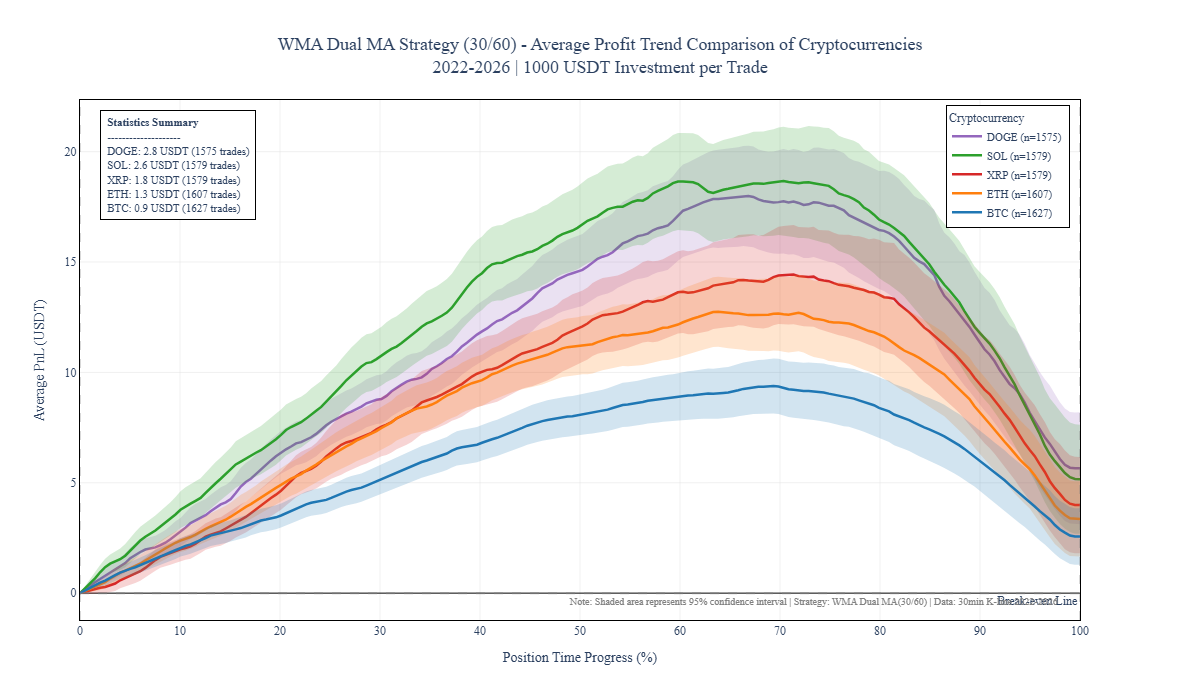
\includegraphics[width=0.85\textwidth]{figs/average_profit_trend.png}
    \caption{Average Profit Paths Across Cryptocurrencies}
    \label{fig:average_profit_trend}
    \vspace{6pt} 
    \parbox{\textwidth}{\small \textit{Note:} This figure illustrates the average trade profit corresponding to each cryptocurrency asset. The horizontal axis denotes the holding duration, while the vertica axis represents profit measured in USDT. The shaded area corresponds to the 95\% confidence interval.}
\end{figure}

Based on the above results, this paper formalizes the phenomenon as unrealized profit drawdown risk and models it as a sequential decision-making problem: during the holding period, how can one determine, based on the current market state and position-related characteristics, whether continued holding will lead to a significant future drawdown in returns, and thereby decide whether the position should be exited early. Unlike traditional approaches that focus on price prediction or trend identification, this paper emphasizes the dynamic evolution of the profit path and its associated risk structure.

We proposes an LSTM-based early-exit decision framework that reformulates the exit problem as a sequence classification task. The framework is designed to be embedded as a data-driven decision layer atop traditional trend-following strategies, learning the optimal exit boundary by balancing future returns and potential drawdowns. Backtesting on cryptocurrency market data demonstrates that the proposed method significantly improves key performance metrics while overall returns remain stable.

The remainder of the paper is organized as follows. Section~\ref{sec:relatedWork} reviews the related literature in this field. Section~\ref{sec:experimental_design} describes the data and displays our strategy and how it works. Section~\ref{sec:results} reports the results of both the baseline strategy and ours, and shows that our LSTM early stopping model outperforms the baseline strategy. Section~\ref{sec:robustness} uses both expanding windows and rolling windows to re-execute the experiment to ensure the robustness of our strategy. Section~\ref{sec:conclusion} concludes the paper and points out future research directions.

\section{Related Work}\label{sec:relatedWork}

Quantitative trading research has long focused on identifying price regularities and transforming them into implementable strategies. The literature has evolved from traditional technical analysis to machine learning–based prediction and, more recently, to reinforcement learning–based sequential decision making. While extensive studies have explored entry signals and price forecasting, optimal exit timing—especially for mitigating unrealized profit drawdown—remains understudied.

\subsection{Trend-following Strategies}

Trend-following represents one of the most classical paradigms in quantitative trading, which exploits price inertia through technical indicators to identify and trade in line with prevailing trends. Moving-average-based methods are the most representative implementations, including the simple moving average (SMA), weighted moving average (WMA), exponential moving average (EMA), and short--long moving-average crossover rules. \citet{Hunter1986} provided an early systematic discussion of the exponentially weighted moving average, emphasizing the importance of recent information in time-series analysis. \citet{Hansun2013} further discussed the evolution and improvement of traditional moving-average tools.

As research developed, scholars began to examine the effectiveness of moving-average rules from theoretical and empirical perspectives rather than treating them as purely empirical tools. \citet{ChiarellaHeHommes2006} analyzed the mechanism of moving-average rules from a dynamic market perspective, noting that window length and trading feedback significantly affect price dynamics. \citet{EllisParbery2005} compared adaptive and simple moving-average strategies, showing that dynamic parameter adjustment improves adaptability. \citet{MarshallNguyenVisaltanachoti2017} compared time-series momentum and moving-average rules, highlighting differences in signal construction and return sources.

Overall, trend-following strategies have evolved from fixed-parameter rules toward adaptive and diversified structures. Traditional technical analysis has not become obsolete with the rise of machine learning; instead, it provides important features for intelligent trading models. For instance, \citet{AyalaEtAl2021} showed that technical strategies are increasingly optimized and integrated via machine learning, enabling a transition from rule-driven to data-driven frameworks.

\subsection{Machine Learning in Trading}

The application of machine learning has significantly transformed the paradigm of quantitative trading. Unlike traditional methods that rely on predefined rules, machine learning automatically captures nonlinear mappings between market data and trading outcomes. Early studies such as \citet{TrippiDeSieno1992} applied neural networks to index futures trading, while \citet{DempsterJones2001} and \citet{DempsterLeemans2006} introduced genetic programming and reinforcement learning, reflecting a shift from manual rule design to automated decision making.

Supervised learning in trading is primarily divided into classification and regression. Classification methods predict price directions or trading signals \citet{ShenJiangZhang2012, GerleinEtAl2016,ZhongEnke2019}, whereas regression methods focus on forecasting price levels and returns \citet{AdegboyeKampouridis2021}.

LSTM has become a milestone in financial time-series modeling due to its ability to capture long-term dependencies. \citet{NelsonPereiraDeOliveira2017} and \citet{FischerKrauss2018} demonstrated its strong performance in direction prediction. \citet{BorovkovaTsiamas2019} extended LSTM to high-frequency data, and \citet{MehtabSenDutta2020,GhoshEtAl2022} further developed hybrid structures combining LSTM with other models.

Recently, machine learning research has shifted from pure prediction accuracy to strategy-oriented performance. \citet{SebastiaoGodinho2021} highlighted that in-sample precision does not guarantee trading profits. \citet{HanKimEnke2023} linked label design more closely with trading system construction, indicating a trend toward profit-driven and strategy-aware modeling.

\subsection{Exit Strategy Optimization}

Compared with entry signal research, exit strategies directly determine profit realization and risk control but have received far less attention. Exit decisions affect not only trade-level PnL but also drawdown management and risk exposure.

Early exit research focused on fixed take-profit and stop-loss rules. \citet{LeungLi2015} ncorporated stop-loss constraints into mean-reversion strategies, emphasizing the impact of exit boundaries on optimality. \citet{LoRemorov2017} showed that stop-loss performance depends heavily on market states. \citet{VezerisKyrgosSchinas2018} found that dynamic volatility-based thresholds outperform fixed ones.

Trailing stop-loss rules further enable profit locking by adjusting exit levels with favorable price movements. \citet{GlynnIglehart1995} provided early theoretical analysis, while \citet{DaiEtAl2021} and \citet{LeungZhang2021} demonstrated their ability to reduce downside risk and formalized trailing stops as optimal stopping problems.

Reinforcement learning has recently emerged as a tool for sequential exit decisions. \citet{KimKim2019}, \citet{TsantekidisEtAl2020}, and \citet{WangEtAl2021} applied deep reinforcement learning to optimize trading boundaries and exit quality. However, such methods remain more focused on overall strategy optimization rather than fine-grained exit timing for individual trades.

Despite progress, research on exit optimization remains limited. \citet{HwangEtAl2023} noted that exit rules strongly influence strategy efficiency, while \citet{SivriEtAl2023} and \citet{Shawky2023} represent early attempts to use machine learning for stop-loss and take-profit calibration. The field still lacks systematic, data-driven frameworks for dynamic exit and drawdown control.

\subsection{Research Gaps}

Existing literature has achieved substantial progress in trend identification, price prediction, and automated trading. However, critical limitations remain in exit optimization, particularly for controlling unrealized profit drawdowns.

First, traditional trend-following strategies rely on fixed parameters and lack robustness to volatile or structurally changing markets. Second, exit research remains underdeveloped relative to entry signal modeling. Studies on trailing exits, dynamic take-profit mechanisms, and integrated exit optimization are especially limited. Third, most studies treat entry, holding, and exit as separate components rather than building a unified decision framework. Poor exit design can erode accurate predictions through profit drawdowns, unnecessary stop-losses, and excessive transaction costs.

In summary, while existing research provides a solid foundation for trend following and machine learning-based prediction, data-driven dynamic exit optimization—especially for profit protection and drawdown control—remains an underexplored area with clear theoretical and practical value.

% \section{Data Description and Preparation}\label{sec:data}

% \subsection{Dataset}

% To objectively evaluate the generalization ability of the LSTM-based early exit decision framework in dynamic market environments, this study selects the cryptocurrency market as the empirical setting. The cryptocurrency market features 24/7 continuous trading, high volatility, and pronounced trend persistence, making it an ideal setting for testing whether the enhanced strategy can effectively improve the traditional trend-following model.

% This study selects four mainstream cryptocurrency trading pairs as the experimental assets: BTC/USDT, ETH/USDT, SOL/USDT, and XRP/USDT, which we collect from the Binance public API. These assets cover different market capitalizations, liquidity characteristics, and price fluctuation patterns, thereby allowing the robustness of the model across assets to be evaluated.

% The raw market data used in the experiment range from January 1, 2022 to March 12, 2026. This interval fully covers multiple bull-bear cycles in the market, enabling the model to be tested across different market regimes, including trend continuation, range-bound fluctuation, and sharp drawdown. In this paper, 30-minute candlestick data are used for modeling. This time granularity ensures the reliability of trend signals while providing sufficient sequence depth for the LSTM model, so as to capture the dynamic evolution of micro risk structures during the holding period.

% We strictly follows the chronological order principle for predictive samples.Based on the trading id we  divides the all the tradings triggered by the baseline strategy into the training set, validation set, and testing set, with proportions of approximately 70\%, 15\%, and 15\%, respectively. The specific sample sizes and corresponding time intervals are shown in Table~\ref{tab:dataset_split}.

% \begin{table}[H]
% \centering
% \caption{Dataset Split}
% \label{tab:dataset_split}
% \small
% \setlength{\tabcolsep}{4pt}
% \renewcommand{\arraystretch}{1.2}
% \begin{tabular}{p{0.15\textwidth}p{0.12\textwidth}p{0.14\textwidth}p{0.18\textwidth}p{0.32\textwidth}}
% \toprule
% Stage & Proportion & Sample Size & Time Interval & Research Function \\
% \midrule
% \makecell{Training\\Set} &
% 70\% &
% 29,250 &
% \makecell{2022/01/02--\\2025/01/06} &
% Model parameter learning and weight optimization \\

% \makecell{Validation\\Set} &
% 15\% &
% 6,268 &
% \makecell{2025/01/06--\\2025/08/05} &
% Hyperparameter tuning and overfitting prevention \\

% \makecell{Testing\\Set} &
% 15\% &
% 6,269 &
% \makecell{2025/08/05--\\2026/03/11} &
% Out-of-sample evaluation and robustness test \\
% \bottomrule
% \end{tabular}
%     \vspace{6pt} 
%     \parbox{\textwidth}{\footnotesize \textit{Note:} Dataset partitioning is based on the total number of trades, with the boundaries strictly defined as $n_{\text{train}} = \lfloor n_{\text{trades}} \times 0.70 \rfloor$ and $n_{\text{val}} = \lfloor n_{\text{trades}} \times 0.15 \rfloor$. Due to the floor truncation operation, a residual fraction of at most one trade is fully allocated to the test set, rendering its actual proportion slightly higher than the theoretical 15\%. Given the large sample size, this deviation accounts for less than 0.5\% of the total data and exerts a negligible impact on evaluation statistics without compromising the integrity of the train/validation boundaries.}
% \end{table}

% \subsection{Data Cleaning}

% This paper first conducts basic cleaning on the raw candlestick data, including uniformly parsing the time field into UTC time format, converting fields such as prices and trading volume into numerical types, and sorting the data in chronological order. Subsequently, anomaly auditing is performed on the raw sequence to identify missing candlesticks, zero-volume candlesticks, and extreme fluctuation samples, with corresponding flags constructed for each type of anomaly. Since the LSTM model adopts a fixed-length historical window for modeling, we further constructs a context-contamination flag using a rolling-window method, and removes samples whose historical windows contain bad data from the training dataset.

\section{Experimental Design}\label{sec:experimental_design}

This paper proposes a deep hybrid decision framework that integrates a traditional trend-following strategy with the risk control capabilities of a deep learning model. The framework is composed of two core components: a baseline layer and a Long Short-Term Memory (LSTM) decision layer. The system operates via a two-layer collaborative mechanism. Specifically, the baseline layer utilizes weighted moving average (WMA) crossover signals\footnote{ For this study, the slow‑period moving average is set to 60 periods, while the fast‑period moving average is set to 30 periods.} and the LSTM decision layer acts as an intelligent risk management module, monitoring market dynamics and generate predicted scores to estimate the likelihood of executing an early exit at each time step, with a position size of 200 USDT per trade. If the predicted score exceeds a predefined threshold, the system enforces a liquidation before the traditional trend-reversal signal occurs, aiming to lock in floating profits or mitigate severe drawdowns. By superimposing a data-driven decision layer onto rule-based logic, this architecture significantly improves the precision of position management during holding periods.The whole model architecture is shown in Figure~\ref{fig:model_architecture}.

\begin{figure}[H]
    \centering
    \includegraphics[width=0.85\textwidth]{figs/model_show.png}
    \caption{Model Architecture}
    \label{fig:model_architecture}
    \vspace{6pt} 
\end{figure}

\subsection{Dataset}

To objectively evaluate the generalization ability of the LSTM-based early exit decision framework in dynamic market environments, this study selects the cryptocurrency market as the empirical setting. The cryptocurrency market features 24/7 continuous trading, high volatility, and pronounced trend persistence, making it an ideal setting for testing whether the enhanced strategy can effectively improve the traditional trend-following model.

This study selects four mainstream cryptocurrency trading pairs as the experimental assets: BTC/USDT, ETH/USDT, SOL/USDT, and XRP/USDT, which we collect from the Binance public API. These assets cover different market capitalizations, liquidity characteristics, and price fluctuation patterns, thereby allowing the robustness of the model across assets to be evaluated.

The raw market data used in the experiment range from January 1, 2022 to March 12, 2026. This interval fully covers multiple bull-bear cycles in the market, enabling the model to be tested across different market regimes, including trend continuation, range-bound fluctuation, and sharp drawdown. In this paper, 30-minute candlestick data are used for modeling. This time granularity ensures the reliability of trend signals while providing sufficient sequence depth for the LSTM model, so as to capture the dynamic evolution of micro risk structures during the holding period.

We strictly follows the chronological order principle for predictive samples.Based on the trading id we  divides the all the tradings triggered by the baseline strategy into the training set, validation set, and testing set, with proportions of approximately 70\%, 15\%, and 15\%, respectively. The specific sample sizes and corresponding time intervals are shown in Table~\ref{tab:dataset_split}.

\begin{table}[H]
\centering
\caption{Dataset Split}
\label{tab:dataset_split}
\small
\setlength{\tabcolsep}{4pt}
\renewcommand{\arraystretch}{1.2}
\begin{tabular}{p{0.15\textwidth}p{0.12\textwidth}p{0.14\textwidth}p{0.18\textwidth}p{0.32\textwidth}}
\toprule
Stage & Proportion & Sample Size & Time Interval & Research Function \\
\midrule
\makecell{Training\\Set} &
70\% &
29,250 &
\makecell{2022/01/02--\\2025/01/06} &
Model parameter learning and weight optimization \\

\makecell{Validation\\Set} &
15\% &
6,268 &
\makecell{2025/01/06--\\2025/08/05} &
Hyperparameter tuning and overfitting prevention \\

\makecell{Testing\\Set} &
15\% &
6,269 &
\makecell{2025/08/05--\\2026/03/11} &
Out-of-sample evaluation and robustness test \\
\bottomrule
\end{tabular}
    \vspace{6pt} 
    \parbox{\textwidth}{\footnotesize \textit{Note:} Dataset partitioning is based on the total number of trades, with the boundaries strictly defined as $n_{\text{train}} = \lfloor n_{\text{trades}} \times 0.70 \rfloor$ and $n_{\text{val}} = \lfloor n_{\text{trades}} \times 0.15 \rfloor$. Due to the floor truncation operation, a residual fraction of at most one trade is fully allocated to the test set, rendering its actual proportion slightly higher than the theoretical 15\%. Given the large sample size, this deviation accounts for less than 0.5\% of the total data and exerts a negligible impact on evaluation statistics without compromising the integrity of the train/validation boundaries.}
\end{table}

\subsection{Data Cleaning}

This paper first conducts basic cleaning on the raw candlestick data, including uniformly parsing the time field into UTC time format, converting fields such as prices and trading volume into numerical types, and sorting the data in chronological order. Subsequently, anomaly auditing is performed on the raw sequence to identify missing candlesticks, zero-volume candlesticks, and extreme fluctuation samples, with corresponding flags constructed for each type of anomaly. Since the LSTM model adopts a fixed-length historical window for modeling, we further constructs a context-contamination flag using a rolling-window method, and removes samples whose historical windows contain bad data from the training dataset.


\subsection{Feature Engineering}

To enable the LSTM decision layer to perceive both the market environment and the current trading state, this paper constructs an input feature system jointly composed of market features and position-context features, providing the informational basis required for the model to identify future unrealized profit drawdown risk.

\subsubsection{Market Features}

When selecting market features, this paper follows the approaches of \citet{FischerKrauss2018}, \citet{HuangWanZhangLu2024}, and \citet{AlKhatibEtAl2022}, and jointly considers price trends, return-generating ability, candlestick patterns, volatility conditions, and trading activity. The detailed definitions of the variables are shown in Table~\ref{tab:market_features}.

\begin{table}[H]
\centering
\caption{Market Features}
\label{tab:market_features}
\small
\renewcommand{\arraystretch}{1.2}
\begin{tabular}{p{0.12\textwidth}p{0.34\textwidth}p{0.43\textwidth}}
\toprule
Category & Feature & Description \\
\midrule
Trend &
\texttt{wma30\_rel}, \texttt{wma60\_rel} &
Deviation of the closing price from the moving averages \\
Trend &
\texttt{wma\_spread} &
Deviation of the 30-day moving average from the 60-day moving average \\
Trend &
\texttt{wma30\_slope}, \texttt{wma60\_slope} &
First-order differences of the moving averages \\
Trend &
\texttt{wma\_spread\_slope} &
The rate of change in the interval between moving averages is used 
to determine their convergence or divergence. \\
Trend &
\texttt{wma\_spread\_accel} &
Acceleration of moving‑average interval variation \\
Strength &
\texttt{ADX(14)} &
Average Directional Index, divided by 100 \\
Momentum &
\texttt{RSI(14)} &
Relative Strength Index, divided by 100 \\
Momentum &
\texttt{MACD\_hist} &
Moving Average Convergence‑Divergence, with fast period 12, slow period 26 and signal 
line period 9, normalized by ATR(14)\\
Return &
\texttt{log\_ret}, \texttt{oc\_rel} &
Log return and open-close ratio \\
Pattern &
\texttt{hl\_range}, \texttt{shadow\_imbalance} &
Price range and upper-lower shadow imbalance \\
Volatility &
\texttt{atr14\_ret} &
ATR(14) divided by the closing price \\
Trading Activity &
\texttt{vol\_z20}, \texttt{taker\_buy\_ratio} &
Trading volume Z-score and active buy ratio \\
\bottomrule
\end{tabular}
\end{table}

\subsubsection{Position Context Features}

% In addition to market features, the key innovation of this paper lies in the introduction of position-context features. Traditional technical indicators usually describe the market itself, but cannot represent the current trading state. However, for the early take-profit problem, the decision implications of the same market trend may differ across different stages of the holding period. For example, the drawdown immediately after opening a position and the drawdown after a large unrealized profit are not equivalent in terms of risk implications. Therefore, this paper represents the position state as model input. The detailed definitions of the variables are shown in Table~\ref{tab:position_context_features}.
A distinguishing methodological contribution of this study is the formal integration of endogenous position-context features alongside conventional exogenous market indicators. While standard technical indicators effectively capture market-wide price dynamics, they fail to represent the ongoing operational state of an active trade. Crucially, the optimal timing for an exit decision is highly path-dependent; the risk implications of an identical market signal can vary significantly across different stages of the holding period. For instance, a price drawdown occurring immediately after position initiation typically indicates an adverse entry or an unfavorable short-term regime. Conversely, an identical drawdown following a substantial unrealized profit signifies a profit give-back that threatens accumulated capital. To reconcile this asymmetry, we incorporate the real-time position state directly into the model's feature space. The detailed definitions of these featuress are presented in Table~\ref{tab:position_context_features}.

\begin{table}[H]
\centering
\caption{Position Context Features}
\label{tab:position_context_features}
\small
\renewcommand{\arraystretch}{1.2}
\begin{tabular}{p{0.25\textwidth}p{0.60\textwidth}}
\toprule
Feature & Description \\
\midrule
\texttt{age} & Number of bars for which the current position has been held transformed by $log$ function to capture the diminishing marginal effect of holding duration \\
\texttt{pnl\_dir} & Unrealized profit or loss in the direction of the position \\
\texttt{mfe} & Maximum favorable excursion \\
\texttt{retrace} & Drawdown from the maximum favorable excursion \\
\bottomrule
\end{tabular}
\end{table}

% By introducing the above position-context information, the LSTM model no longer makes decisions solely based on market states, but is able to make decisions according to the dynamic profit and loss condition of the current trade, the holding duration, and other information. This allows the model to more closely approximate the risk-management logic of real trading.
By augmenting the feature space with these position-context variables, the exit decision framework shifts from a conventional price-forecasting mechanism to a joint state-space optimization problem. The LSTM network is thus equipped to evaluate exogenous market fluctuations conditional on the internal lifecycle of the trade (e.g., holding duration, trailing drawdown from peak equity). Consequently, this feature architecture allows the deep learning model to more closely replicate the conditional risk-management logic executed by professional traders, optimizing the trade-off between trend-following endurance and capital preservation.

\subsection{Training Stage}\label{subsec:training_stage}

\textbf{Grid Search:} First, we employ a grid search to determine the optimal model parameters. The parameters to be optimized include the drawdown penalty coefficient ($\lambda_{dd}$, an important parameter which we illustrate in Appendix~\ref{sec:drawdownpenalty}), the rolling window length, the number of neural network layers, and the early exit decision threshold ($\theta$). We define a discrete search space for these parameters, generating multiple parameter combinations where each corresponds to a distinct model. Subsequently, we train these models individually and evaluate their performance on the validation set to select the top five best-performing models.The scoring mechanism comprehensively considers the Sharpe ratio, the average profit per trade, and the maximum drawdown. We employ the entropy weight method to integrate these three metrics to derive the final evaluation score for the models.

During this process, only models that satisfy the following three strict filtering conditions in the valid set will be retained:

First, the early exit rate must be strictly less than 65\% to prevent the model from executing premature exits excessively. It is designed to prevent the model from converging to a degenerate solution driven by excessive risk aversion. Because the loss function heavily penalizes drawdowns, the LSTM network tends to minimize training loss by prematurely liquidating positions at the slightest market fluctuation. Imposing this upper bound acts as a behavioral regularization that forces the model to identify genuine risk boundaries rather than simply avoiding risk through constant exits, thereby preserving the strategy's underlying trend-following logic and profitability. Second, the model's total return must exceed 80\% of the total return generated by the baseline strategy, ensuring that the model's performance does not significantly underperform the baseline. Finally, the maximum drawdown must be less than 150 USDT. Given the previously mentioned position size of 200 USDT per trade, this maximum drawdown corresponds to a maximum loss of 75\%. Exceeding this threshold indicates that the strategy has suffered consecutive severe losses within a short period, implying that the model's exit decisions not only failed to protect profits but actually exacerbated the losses.The score distribution of the eligible models are displayed in Appendix~\ref{subsec:scoresDistribution} and the performance of the top five best-performing models on the validation set is presented in Appendix~\ref{subsec:gridsearch}.

\textbf{Label Construction and Adaptive Margin Setting:} To train the LSTM decision layer, a binary supervisory label is constructed for each timestamp during the holding period. Here, $\Delta_{\text{margin}}$ serves as the core parameter for label definition in this system. AK line is labeled as a positive sample only if the floating return of the current bar exceeds the final return by at least $\Delta_{\text{margin}}$. Consequently, the value of $\Delta_{\text{margin}}$ directly dictates the proportion of positive samples, which in turn influences the exit propensity learned by the model. When the value is too small, numerous marginal samples are labeled as positive, causing the model to frequently trigger premature exit signals. Conversely, an excessively large value leads to an extreme scarcity of positive samples, biasing the model towards non-execution and rendering the early exit mechanism ineffective.

Empirically, constraining the positive sample ratio to approximately $0.35$ yields robust model performance. Based on this target ratio, the preliminary $\Delta_{\text{margin}}$ values computed for each asset are: $0.008$ for ETH, $0.006$ for BTC, $0.012$ for SOL, and $0.008$ for XRP. After establishing these initial values, we utilize the top three optimal parameter combinations identified from the preceding grid search to conduct an ablation study. Specifically, we define a set of candidate $\Delta_{\text{margin}}$ values covering a spectrum from lenient to strict ($0.003$, $0.005$, $0.008$, $0.010$, $0.012$, and $0.015$). By exclusively varying $\Delta_{\text{margin}}$, we re-evaluate the model's performance across several key metrics: the positive sample ratio, the validation return versus the baseline strategy return, the Sharpe ratio, and the early exit trigger rate. The cross-asset results of this ablation analysis are detailed in Appendix~\ref{subsec:ablationAnalysis}.

To ensure that the selected optimal parameters are not an artifact of overfitting, we conduct a sensitivity analysis on the corresponding parameters for each asset, with the results detailed in Appendix~\ref{subsec:sensitivityAnalysis}. The findings indicate that the model's performance does not exhibit high sensitivity to minor variations across the parameters; specifically, no abrupt "isolated peaks" are observed in the plots. The sensitivity analysis for BTC and ETH is particularly robust, suggesting that large-cap cryptocurrencies are relatively insensitive to parameter fluctuations.

% \textbf{Dropout Regularization:} To prevent the model from overfitting on the training set, dropout is introduced as a structural regularization technique between the LSTM layers and the fully connected (FC) layer. The initial dropout rate is set to $0.2$, serving as a fixed value during the first stage, and is subjected to an ablation study following the completion of the primary grid search.

% In terms of experimental design, a two-tier dropout mechanism is implemented at distinct positions. The first tier is the inter-layer dropout, applied between adjacent LSTM layers to randomly mask connections during each forward pass. The second tier is the output dropout, applied between the final hidden state output of the LSTM and the FC layer, ensuring that the regularization remains effective under both single-layer and multi-layer network configurations.

% In the second stage, an ablation study is conducted specifically on the dropout rate. Using the initial dropout rate as an empirical baseline, the optimal parameter combination is fixed after the primary grid search. We then define a candidate set of dropout rates as $\{0.1, 0.2, 0.3\}$ and re-evaluate the model's performance under each setting. The performance evaluation metric is identical to that defined in Equation~\ref{eq:performanceMetric}.

\subsection{LSTM Model}

We adopts a Long Short-Term Memory (LSTM) network as the early-exit decision model. LSTM is suitable for capturing dynamic dependence in financial time series and can, to a certain extent, capture the nonlinear relationship between trend evolution and position-state changes.

The model input is a fixed-length historical feature matrix which we mentioned before:

\begin{equation}
    \mathbf{X}_{t-m+1:t} \in \mathbb{R}^{m \times n}
\end{equation}

where $m$ denotes the length of the time window, and $n$ denotes the feature dimension contained in each time step.

The LSTM model recursively encodes the input sequence and uses the hidden state of the last time step as a comprehensive representation of the current holding state. The hidden state is then mapped into a one-dimensional output through a fully connected layer and converted into a probability form through the Sigmoid function:

\begin{equation}
    p_t = \sigma(\mathbf{w}\mathbf{h}_t + b)
\end{equation}

where $\mathbf{h}_t$ denotes the hidden state of the LSTM at the current time, $\mathbf{w}$ and $b$ denote the weight and bias of the fully connected layer, respectively, and $\sigma(\cdot)$ denotes the Sigmoid activation function. 

% \begin{equation}
%     p_t = P(y_t = 1 \mid \mathbf{X}_{t-63:t})
% \end{equation}

When $p_t$ is close to 1, it indicates that the model believes the future unrealized profit drawdown risk is relatively high and that the current position should be closed early. When $p_t$ is close to 0, it indicates that continuing to hold the position is more reasonable.

\subsection{Decision Rule}

In the backtesting stage, the LSTM decision layer operates as an additional exit module on top of the baseline strategy. The baseline strategy still generates trading directions and initial entry signals, while the LSTM model participates in decision-making only when an existing position is being held.

Specifically, when the system executes a WMA crossover rule based on the baseline strategy and establishes a position, for each new candlestick, the market features and position-context features are updated, and the feature sequence of the most recent window is input into the LSTM model to obtain the early-exit predicted score $p_t$.

The exit rule in this paper can be expressed as:

\begin{equation}
    Exit_t =
    \begin{cases}
    1, & p_t > \theta \\
    -1, & \text{opposite WMA crossover occurs} \\
    0, & \text{else}
    \end{cases}
\end{equation}

where $\theta$ is the decision threshold for early exit, determined through grid search. When $p_t > \theta$, it indicates that the model judges the current position to face a relatively high future unrealized profit drawdown risk, and therefore the system will actively close the position before the reverse crossover signal of the baseline strategy appears. If the LSTM does not trigger an early exit, the trade continues to be managed according to the original moving-average reverse crossover rule.

Through the above decision rule, this paper forms a two-layer exit mechanism: the baseline strategy provides trend-reversal exits, while the LSTM layer provides risk-warning-based early exits. The former ensures that the strategy still follows trend-following trading logic, while the latter improves the responsiveness to unrealized profit drawdown risk during the holding period. This mechanism enables the strategy to no longer passively wait for the moving-average reverse crossover, but instead to lock in profits in advance when drawdown risk rises, thereby improving strategy performance.

\subsection{Comparison Models}\label{subsec:comparison_models}

To evaluate the effectiveness of the proposed LSTM-based early exit framework in enhancing returns and controlling drawdowns, its performance is compared against two representative benchmark strategies. The first is the underlying WMA baseline strategy, which acts as the fundamental trend-following reference utilizing 30-day and 60-day weighted moving averages without any auxiliary exit mechanism. The second is the simple buy-and-hold strategy. This comparative analysis allows us to observe whether the proposed model can significantly outperform the existing benchmark strategies, thereby validating its superiority in dynamic risk identification.

In terms of experimental design, all strategies are uniformly applied to multiple mainstream cryptocurrency trading pairs, specifically BTC/USDT, ETH/USDT, SOL/USDT, and XRP/USDT. Conducting these cross-asset experiments under identical parameters allows for a comprehensive assessment of the robustness and generalizability of the proposed framework across diverse market structures.

\section{Results}\label{sec:results}

Based on the validation set performance, we identify the optimal parameter combinations for each asset (see Table~\ref{tab:optimal_parameters}). For each parameter combination, we backtest the proposed strategy using the test set data coverd from Jul 28, 2025 to Mar 12,2026 to evaluate the out-of-sample performance of the corresponding model. Furthermore, to benchmark the performance enhancements achieved by our framework, we concurrently evaluate the baseline WMA strategy and the buy-and-hold strategy to analyze the relative improvements.

\begin{table}[H]
  \centering
  \caption{Optimal Hyperparameter Configurat  ion for Each Asset}
  \label{tab:optimal_parameters}
  \small
  \begin{tabular}{cccccc}
    \toprule
    \textbf{Asset} & \textbf{Window Size} & $\boldsymbol{\lambda_{dd}}$ & \textbf{Num Layers} & $\boldsymbol{\theta}$ & \textbf{Seed} \\
    \midrule
    ETH & 96 & 2.0 & 1 & 0.6 & 42 \\
    BTC & 32 & 1.0 & 2 & 0.5 & 456 \\
    XRP & 64 & 2.0 & 2 & 0.6 & 123 \\
    SOL & 32 & 1.5 & 1 & 0.5 & 123 \\
    \bottomrule
  \end{tabular}
  \vspace{6pt}
  \parbox{0.85\textwidth}{\footnotesize \textit{Note:} This table presents the optimal parameter combination for each asset. Specifically, Window Size denotes the lookback window length, $\lambda_{dd}$ represents the drawdown penalty coefficient, Num Layers indicates the number of neural network layers, $\theta$ denotes the early exit decision threshold, and Seed is the random seed.}
\end{table}

Figure~\ref{fig:merged_cum_pnl_total} illustrates the cumulative returns of the combination of the top optimal LSTM early exit models, the baseline WMA strategy, and the buy-and-hold strategy for each asset. As can be observed, both the early exit models and the baseline WMA strategy significantly outperform the buy-and-hold strategy in terms of cumulative returns. With the exception of SOL, the LSTM early exit models demonstrate a substantial improvement over the baseline strategy across the other three cryptocurrencies.
% The cumulative returns of each LSTM early exit strategy are detailed in Appendix~\ref{subsec:LSTM_Early_Stopping_Details}.

\begin{figure}[H]
    \centering
    
\includegraphics[width=0.85\textwidth]{figs/Merged_Coins_cummupnl_total.png}
    \caption{Total Cumulative Returns of Different Strategies for Each Asset}
    \label{fig:merged_cum_pnl_total}
    \vspace{6pt} 
    \parbox{0.85\textwidth}{\footnotesize \textit{Note:} The solid blue line represents the cumulative returns of the combination of the optimal LSTM early exit models, the dashed line represents the baseline WMA strategy, and the solid orange line represents the buy-and-hold strategy. The shaded area indicates the outperformance (or underperformance) of the early exit models relative to the baseline strategy.}
\end{figure}

% In addition to cumulative returns, we evaluate the model performance based on the Sharpe ratio and the early exit probability. Appendix~\ref{subsec:Test_Set_Metrics} presents the performance metrics of the top three optimal LSTM early exit models and the baseline WMA strategy for each asset. As can be observed, for every asset, at least one LSTM early exit model significantly outperforms the baseline strategy. This demonstrates that our proposed model can indeed improve performance on top of the baseline strategy; however, it also indicates that the model's performance is relatively sensitive to parameter settings.

% To further examine the per-trade profitability across different strategies, we employ box plots to visualize the profit distribution of individual trades, as illustrated in Figure~\ref{fig:merged_perTradeDistribution}.As can be observed, the early exit models exhibit an elevated mean value in the box plots relative to the baseline strategy, indicating an improvement in average profitability.

% \begin{figure}[H]
%     \centering
%     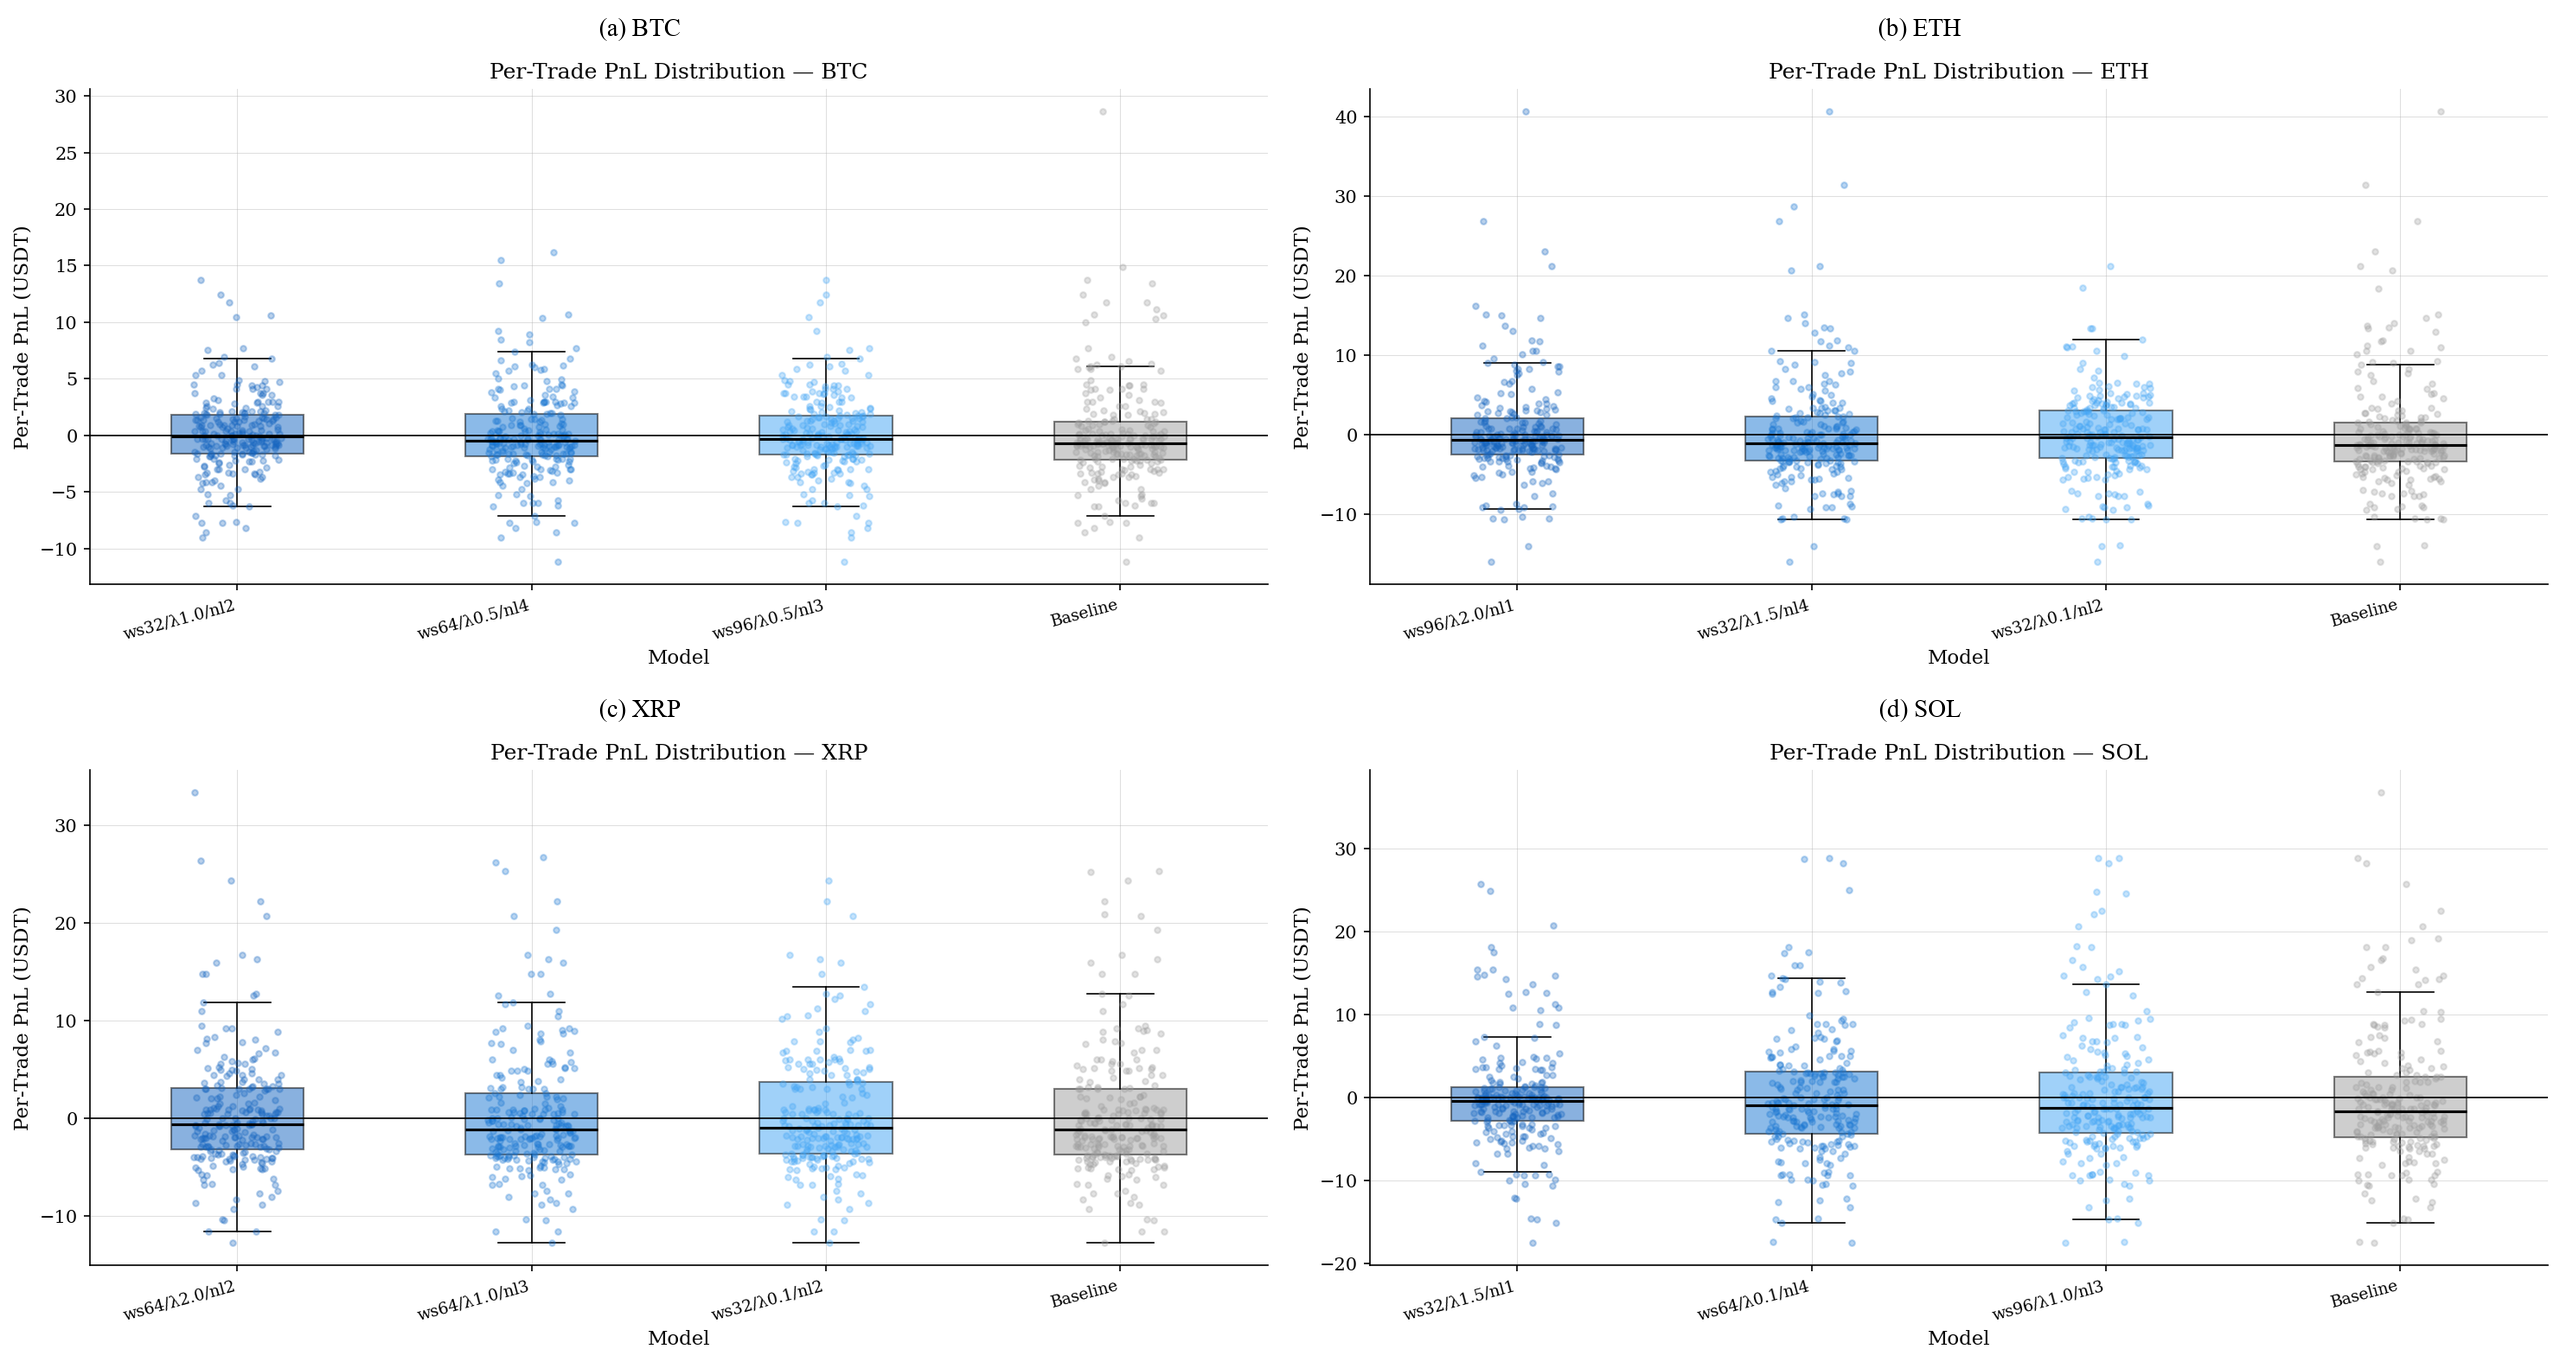
\includegraphics[width=0.85\textwidth]{figs/Merged_Coins_perTradeDistribution.png}
%     \caption{Profit Distribution of Different Strategies for Each Asset}
%     \label{fig:merged_perTradeDistribution}
%     \vspace{6pt} 
%     \parbox{0.85\textwidth}{\footnotesize \textit{Note:} The box plot displays the profit distribution of each strategy for each asset.}
% \end{figure}

Furthermore, as previously noted in Section~\ref{sec:introduction}, a majority of trades experience a profitable state at some point during the holding period but ultimately close at a loss. To investigate whether the proposed model improves the trade-level win rate, we categorize each trade into one of four outcomes relative to the baseline strategy across each asset: (i) winning in both strategies (Kept Win), (ii) losing in both strategies (Kept Loss), (iii) converted from a baseline loss to an LSTM profit (Turned Win), and (iv) converted from a baseline profit to an LSTM loss (Turned Loss). The results are shown in Figure~\ref{fig:improve_on_winrate} and Table~\ref{tab:transition_summary}.

\begin{figure}[H]
    \centering
    
\includegraphics[width=0.85\textwidth]{figs/improve_on_winrate.png}
    \caption{Distribution of Trade Outcomes Relative to the Baseline Strategy for Each Asset}
    \label{fig:improve_on_winrate}
    \vspace{6pt}   
    \parbox{0.85\textwidth}{\footnotesize \textit{Note:} These pie charts illustrate the win rates of the baseline strategy and the optimal LSTM early exit strategies for each asset. Specifically, the blue areas represent trades that win in both strategies (Kept Win), and the gray areas represent trades that lose in both strategies (Kept Loss). The green areas indicate trades converted from a baseline loss to an LSTM profit (Turned Win), while the red areas denote trades converted from a baseline profit to an LSTM loss (Turned Loss).}
\end{figure}

\begin{table}[H]
\centering
\caption{Win/Loss Transition Summary Across Assets}
\label{tab:transition_summary}
\begin{tabular}{llccc}
\toprule
Asset & Model & Win Rate & Turned Win & Turned Loss \\
\midrule

\multirow{2}{*}{ETH} 
& Baseline              & 34.7\% & ---         & ---        \\
& ws96/$\lambda$2.0/nl1 & 38.1\% & 15 (6.4\%)  & 7 (3.0\%)  \\
\addlinespace

\multirow{2}{*}{BTC} 
& Baseline              & 35.6\% & ---         & ---        \\
& ws32/$\lambda$1.0/nl2 & 48.1\% & 34 (14.2\%) & 4 (1.7\%)  \\
\addlinespace

\multirow{2}{*}{XRP} 
& Baseline              & 38.4\% & ---         & ---        \\
& ws64/$\lambda$2.0/nl2 & 44.6\% & 16 (6.9\%)  & 1 (0.4\%)  \\
\addlinespace

\multirow{2}{*}{SOL} 
& Baseline              & 34.9\% & ---         & ---        \\
& ws32/$\lambda$1.5/nl1 & 40.5\% & 27 (11.6\%) & 14 (6.0\%) \\

\bottomrule
\end{tabular}
\end{table}

\section{Robustness Checks}\label{sec:robustness}

\textbf{Expanding Window Training:}In the main experiment, the training, validation, and test sets all utilized fixed window lengths. In this study, we employ a expanding-window training method. The initial training set is set to 2020.01--2021.05, the validation set to 2021.05--2021.11, and the test set to 2021.11--2022.06. Thereafter, we extend the sample forward using a 6-month step size, maintaining a consistent ratio of 70\%, 15\%, and 15\% for the training, validation, and test sets within each sample group. The detailed progression is presented in Table~\ref{tab:dataset_windows}.

\begin{table}[H]
  \centering
  \setlength{\tabcolsep}{3pt}
  \caption{Dataset Partitioning Across Expanding Windows}
  \label{tab:dataset_windows}
  \small
  \begin{tabular}{lcccc}
    \toprule
    \textbf{Window} & \textbf{Data Period} & \textbf{Training Set (70\%)} & \textbf{Validation Set (15\%)} & \textbf{Test Set (15\%)} \\
    \midrule
    Window 1 & 2020.01--2022.06 & 2020.01--2021.05 & 2021.05--2021.11 & 2021.11--2022.06 \\
    Window 2 & 2020.01--2023.01 & 2020.01--2022.03 & 2022.03--2022.09 & 2022.09--2023.01 \\
    Window 3 & 2020.01--2023.07 & 2020.01--2022.09 & 2022.09--2023.02 & 2023.02--2023.07 \\
    Window 4 & 2020.01--2024.01 & 2020.01--2023.03 & 2023.03--2023.09 & 2023.09--2024.01 \\
    Window 5 & 2020.01--2026.03 & 2020.01--2024.04 & 2024.04--2025.01 & 2025.01--2026.03 \\
    \bottomrule
  \end{tabular}
  \vspace{6pt}
  \parbox{\textwidth}{\footnotesize \textit{Note:} This table presents the temporal boundaries for the expanding data windows. Window 5 represents the original complete dataset. Each window is strictly partitioned chronologically into a training set, a validation set, and a test set to evaluate the out-of-sample robustness of the model across different market periods.}
\end{table}

Due to the substantial interference from controversial information regarding XRP and SOL in their early years, we exclude these two assets upon expanding the sample window. The acumulative profitability and Sharpe ratio of the strategies across the test sets of each expanding window for ETH and BTC are illustrated in Figure~\ref{fig:wfa}.

\begin{figure}[H]
    \centering
    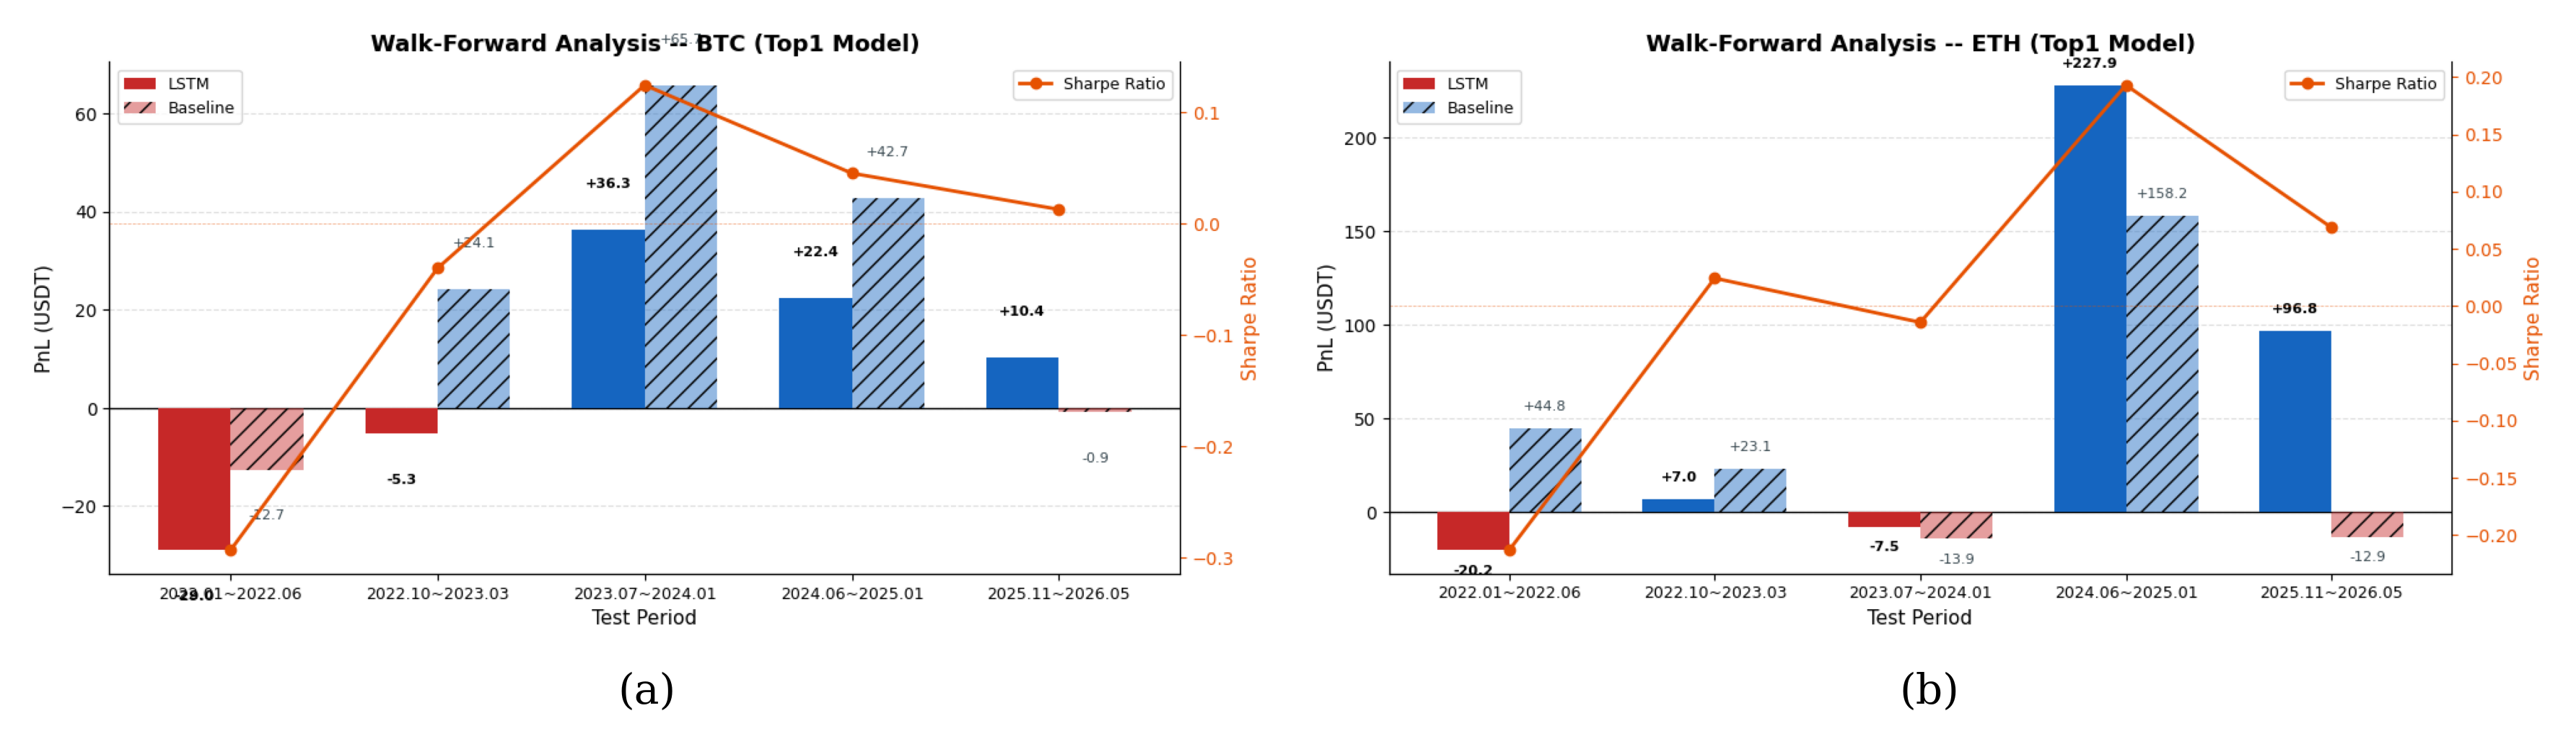
\includegraphics[width=0.85\textwidth]{figs/wfa.png}
    \caption{Average Profit/Loss of Different Models for ETH and BTC:Expanding Windows}
    \label{fig:wfa}
    \vspace{6pt}   
    \parbox{0.85\textwidth}{\footnotesize \textit{Note:} Panels (a) and (b) present the average profitability under different periods for BTC and ETH using expanding windows, respectively. The orange lines depict the Sharpe ratios of the LSTM early exit models across different configurations. The solid (untextured) bars represent the average profitability of the LSTM early exit models, while the textured bars denote the average profitability of the baseline WMA strategy.}
\end{figure}  

As can be observed from the figure, for BTC, the LSTM early exit models underperform the baseline strategy in all but the most recent sample window. In the fifth window, the average profitability of the baseline strategy is -0.9 USDT, whereas the LSTM early exit model achieves an average profitability of 10.4 USDT. In contrast, for ETH, the LSTM early exit models consistently outperform the baseline strategy across the three most recent windows, indicating that our proposed strategy indeed delivers significant performance improvements. Specifically, from the third to the fifth window, the average profitability of the LSTM early exit models is -7.5 USDT, 227.9 USDT, and 96.8 USDT, respectively, while the corresponding baseline strategy yields only -13.9 USDT, 158.2 USDT, and -12.9 USDT, respectively.

\textbf{Rolling Window Training:} However, the expanding window approach assumes that market conditions remain constant over the long term. In reality, market dynamics are inherently time-varying. Therefore, we employ a rolling window approach to capture these changing market dynamics and to examine whether our proposed strategy can continue to significantly outperform the baseline strategy under this framework. We similarly conducted five sets of tests, and the results are illustrated in Figure~\ref{fig:wfa_roll}.

\begin{figure}[H]
    \centering
    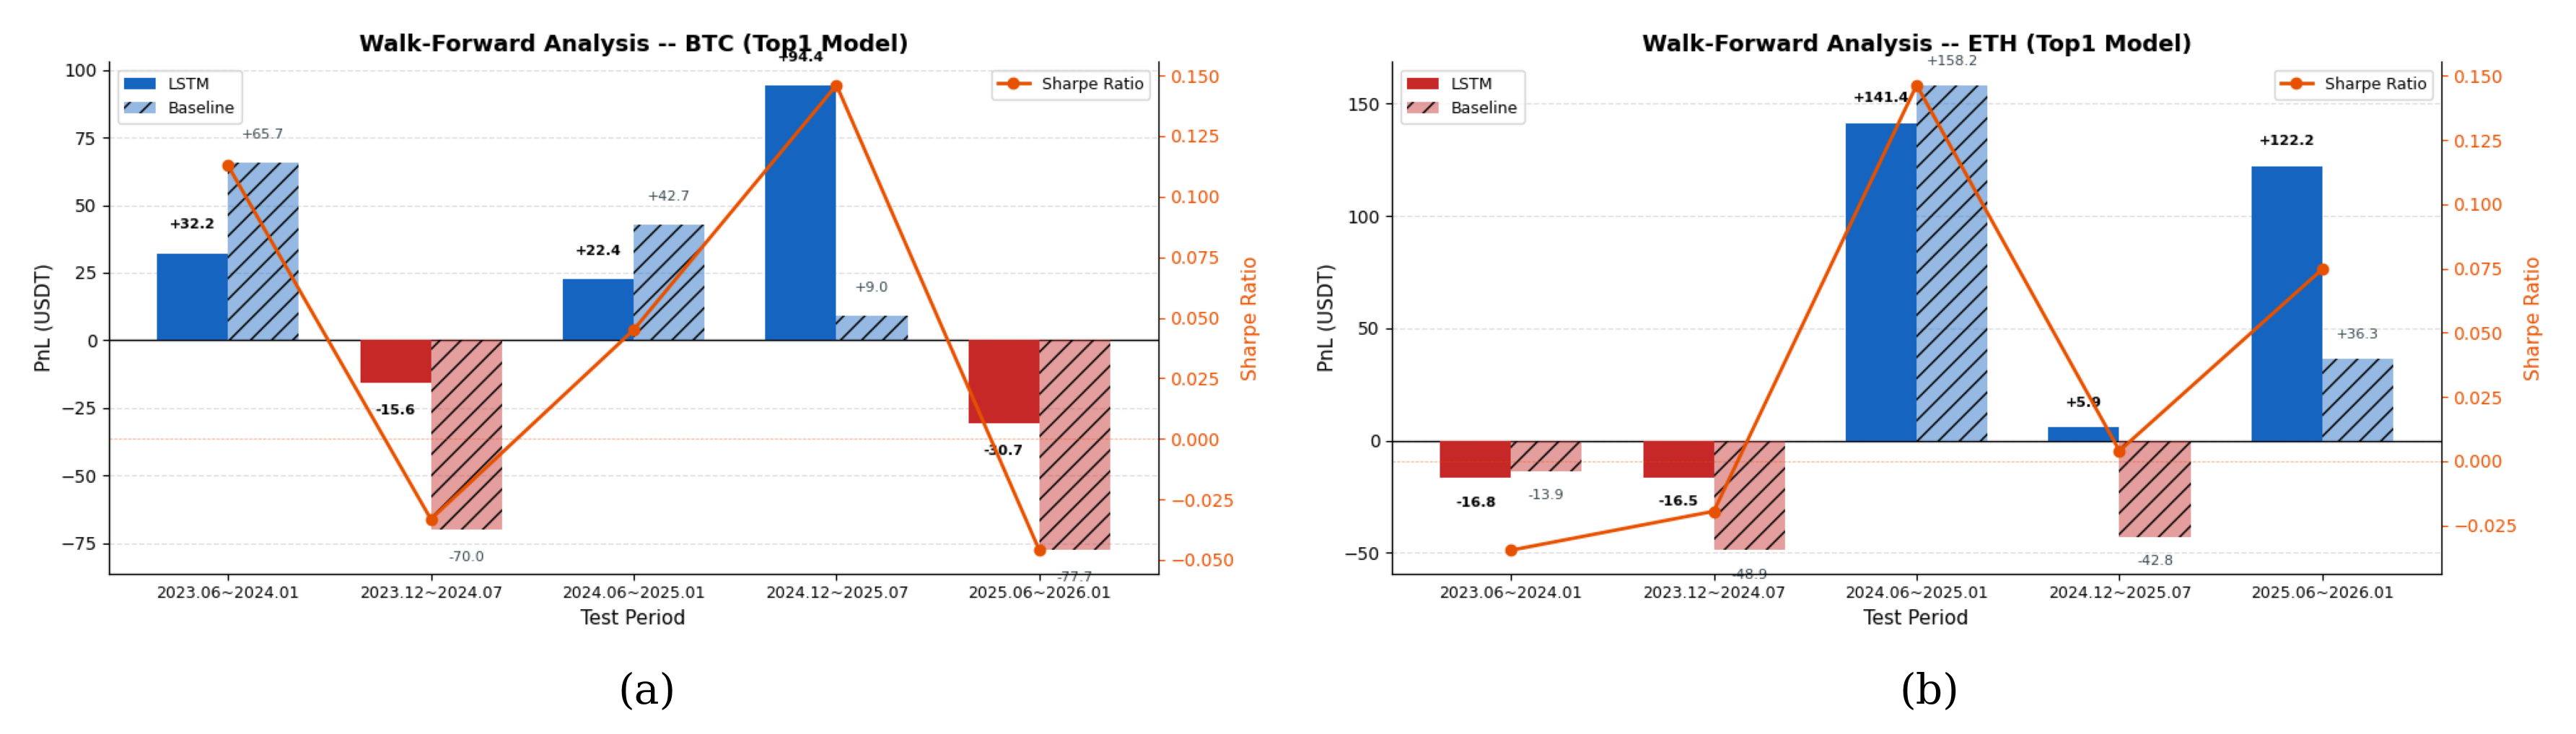
\includegraphics[width=0.85\textwidth]{figs/wfa_roll.png}
    \caption{Average Profit/Loss of Different Models for ETH and BTC:Robustness}
    \label{fig:wfa_roll}
    \vspace{6pt}   
    \parbox{0.85\textwidth}{\footnotesize \textit{Note:} Panels (a) and (b) present the average profitability under different periods for BTC and ETH using rolling windows, respectively. The orange lines depict the Sharpe ratios of the LSTM early exit models across different configurations. The solid (untextured) bars represent the average profitability of the LSTM early exit models, while the textured bars denote the average profitability of the baseline WMA strategy.}
\end{figure}  

Upon switching to the rolling window approach, we find that the overall performance of the LSTM early exit models on ETH is consistent with that on BTC; for both assets, the early exit models outperform the baseline strategy in three out of the five test windows. Furthermore, we observe that when the acumulative profitability of the baseline strategy is significantly negative, the LSTM early exit models can achieve positive returns or incur substantially smaller losses. For instance, for BTC, the baseline strategy incurs losses of -70.0 USDT and -77.7 USDT in the second and fifth windows, respectively, whereas our models limit the losses to merely -15.6 USDT and -30.7 USDT, respectively. This demonstrates that the underlying mechanism by which our proposed strategy improves upon the baseline strategy is not solely locking in profits, but more importantly, executing timely stop-losses.

\section{Conclusion and Future Work}\label{sec:conclusion}

The dual-layer framework, which combines a baseline WMA entry rule with an LSTM-based exit policy, significantly outperforms both the standalone baseline strategy and the passive buy-and-hold benchmark. Out-of-sample testing shows substantial improvements in cumulative returns and Sharpe ratios across the majority of tested assets, specifically BTC, ETH, and SOL.

By incorporating transaction-level position-context features—specifically maximum favorable excursion (MFE) and trailing drawdown—the LSTM model successfully identifies trend exhaustion before a moving average crossover occurs. This early liquidation mechanism effectively addresses the inherent lag of traditional exit rules and protects accumulated paper profits.

Granular per-trade PnL analysis indicates that the LSTM exit system alters the return profile in an asymmetric manner. The framework effectively curtails the downside risks and shifts the median of trade returns upward, while successfully preserving the right-tail gains generated by major macroscopic trends.

While the proposed LSTM exit system delivers robust performance, several avenues remain open for future research. First, while our backtesting accounts for baseline execution costs, the impact of varying market liquidity, slippage, and alternative fee structures under hyper-volatile regimes warrants a more accurate microstructure analysis. Second, the current framework operates on an asset-by-asset basis; extending this dual-layer architecture to a multi-asset portfolio level—incorporating dynamic capital allocation and cross-asset risk spillovers—could further smooth the equity curve. Finally, incorporating Deep Reinforcement Learning (DRL) to jointly optimize entry, sizing, and exit decisions within an end-to-end continuous control environment represents a promising technological advancement over the discrete probability-threshold approach.








\newpage

% =========================
% References
% =========================
\bibliographystyle{apalike}
\bibliography{references}

\newpage

% =========================
% Appendix
% =========================
\appendix

\section{Illustration on Drawdown Penalty Coefficient}\label{sec:drawdownpenalty}

To align the neural network's optimization objective with the real-world risk management goals of trend-following strategies, we introduce an asymmetric loss function. Standard Binary Cross-Entropy (BCE) loss treats False Positives (premature exits) and False Negatives (missed drawdown protections) symmetrically. However, in quantitative trading, the financial penalty of failing to capture a severe profit give-back is substantially higher than the opportunity cost of a slightly premature liquidation. 

Therefore, during the training phase, we employ a Weighted Binary Cross-Entropy loss governed by the drawdown penalty coefficient ($\lambda_{dd}$). Formally, for a given training sequence at time $t$, the loss function is defined as:

\setcounter{equation}{0}
\renewcommand{\theequation}{A.\arabic{equation}}

\begin{equation}
\mathcal{L} = - \frac{1}{N} \sum_{i=1}^{N} \left[ \lambda_{dd} \cdot y_i \log(p_i) + (1 - y_i) \log(1 - p_i) \right]
\end{equation}

where $y_i \in \{0, 1\}$ represents the binary supervisory label of early exit, and $p_i$ is the conditional probability predicted by the LSTM layer. 

The hyperparameter $\lambda_{dd} > 0$ acts as a financial risk-aversion multiplier. When $\lambda_{dd} > 1.0$, the gradient update heavily penalizes the model for failing to predict an early exit when a substantial trailing drawdown is imminent ($y_i = 1$). Economically, tweaking $\lambda_{dd}$ allows our framework to adapt to different market microstructures and accommodate traders with varying degrees of drawdown tolerance.

\section{Additional Figures}

\subsection{Model Scores Across Different Parameter Configurations for Each Asset}\label{subsec:scoresDistribution}

\begin{figure}[H]
    \centering
    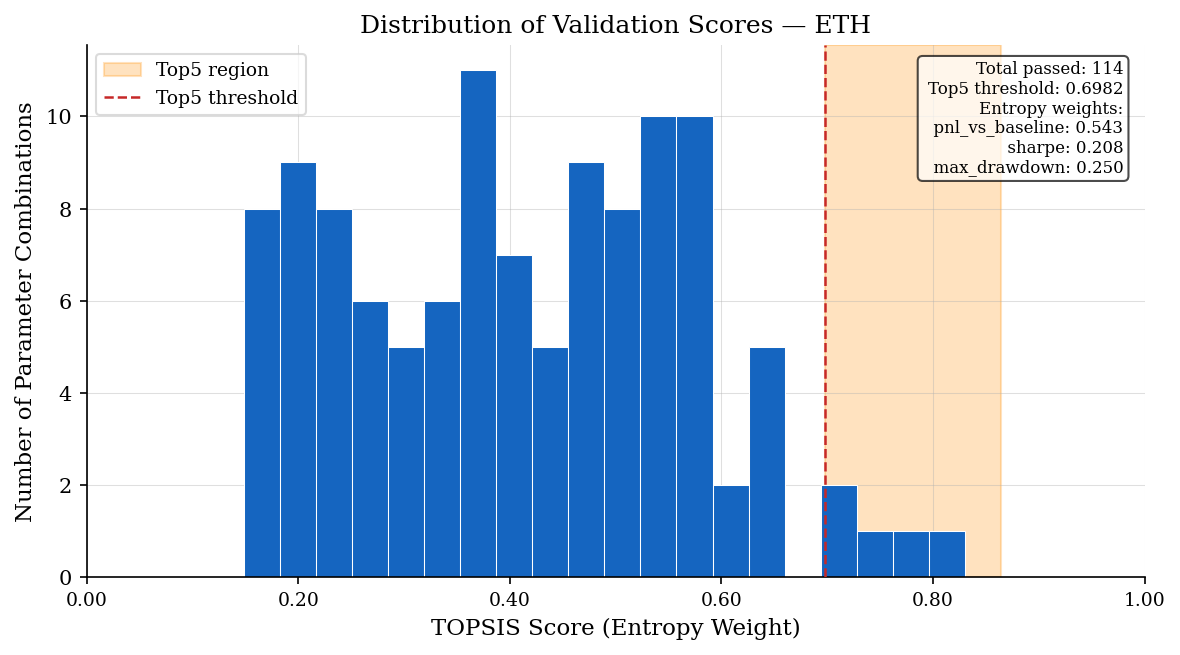
\includegraphics[width=0.85\textwidth]{figs/score_eth.png}
    \caption{Model Scores Across Different Parameter Configurations for ETH}  
    \label{fig:scores_eth}
    \vspace{6pt} 
    \parbox{0.85\textwidth}{\footnotesize \textit{Note:} This figure presents the model scores across different parameter configurations for ETH. The orange shaded area indicates the region corresponding to the top five models.}
\end{figure}

\begin{figure}[H]
    \centering
    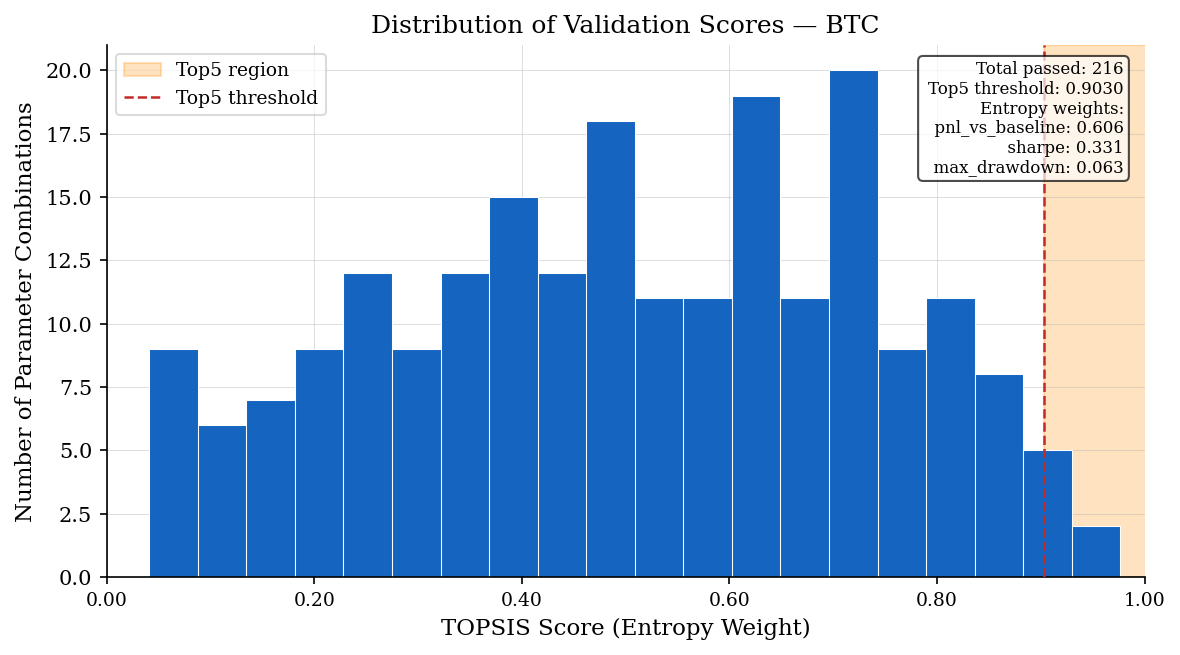
\includegraphics[width=0.85\textwidth]{figs/score_btc.png}
    \caption{Model Scores Across Different Parameter Configurations for BTC}  
    \label{fig:scores_btc}
    \vspace{6pt} 
    \parbox{0.85\textwidth}{\footnotesize \textit{Note:} This figure presents the model scores across different parameter configurations for BTC. The orange shaded area indicates the region corresponding to the top five models.}
\end{figure}

\begin{figure}[H]
    \centering
    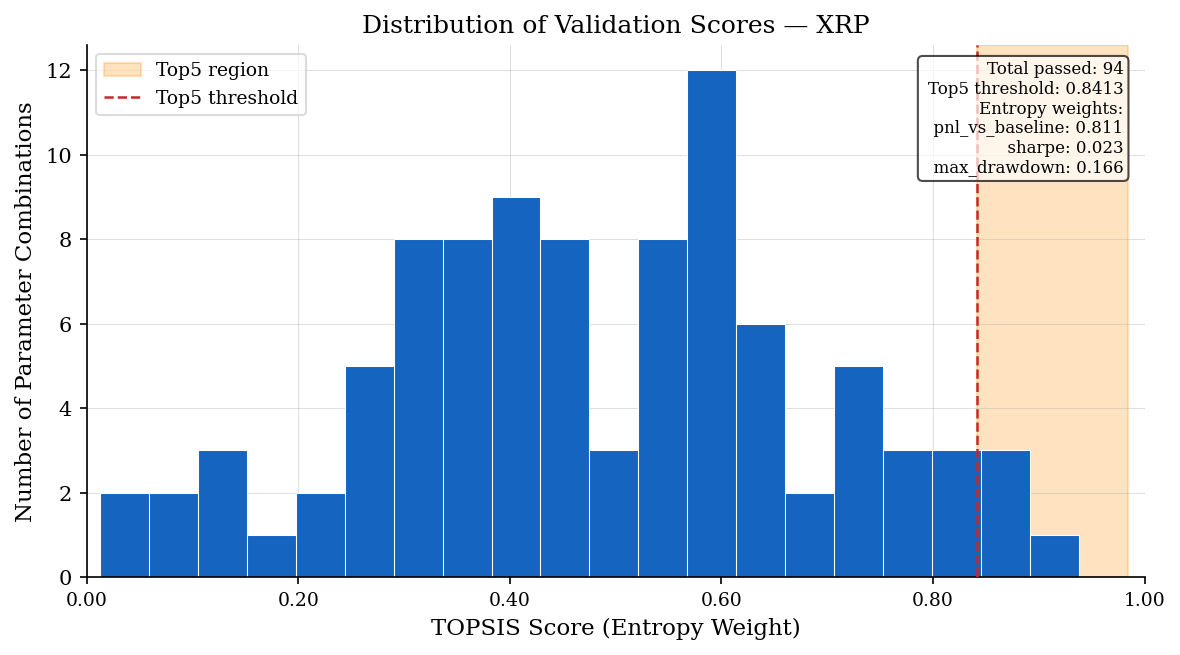
\includegraphics[width=0.85\textwidth]{figs/score_xrp.png}
    \caption{Model Scores Across Different Parameter Configurations for XRP}  
    \label{fig:scores_xrp}
    \vspace{6pt} 
    \parbox{0.85\textwidth}{\footnotesize \textit{Note:} This figure presents the model scores across different parameter configurations for XRP. The orange shaded area indicates the region corresponding to the top five models.}
\end{figure}

\begin{figure}[H]
    \centering
    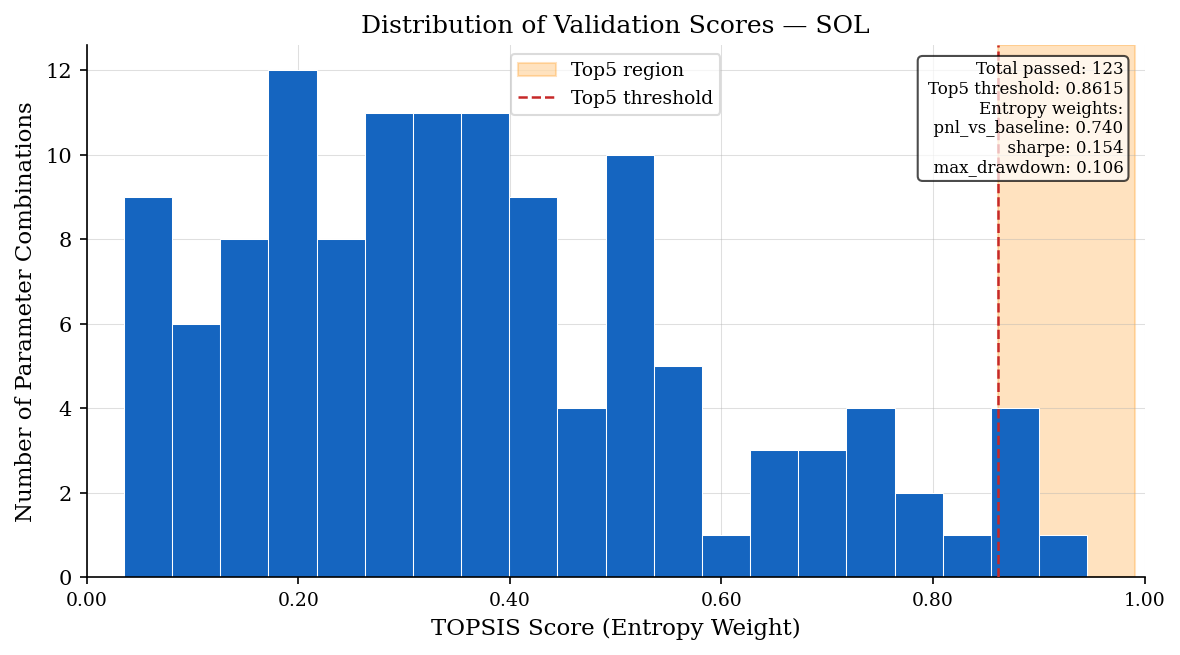
\includegraphics[width=0.85\textwidth]{figs/score_sol.png}
    \caption{Model Scores Across Different Parameter Configurations for SOL}  
    \label{fig:scores_sol}
    \vspace{6pt} 
    \parbox{0.85\textwidth}{\footnotesize \textit{Note:} This figure presents the model scores across different parameter configurations for SOL. The orange shaded area indicates the region corresponding to the top five models.}
\end{figure}

\subsection{Validation Set Metrics of Top Five Models for Each Assets}\label{subsec:gridsearch}

\begin{figure}[H]
    \centering
    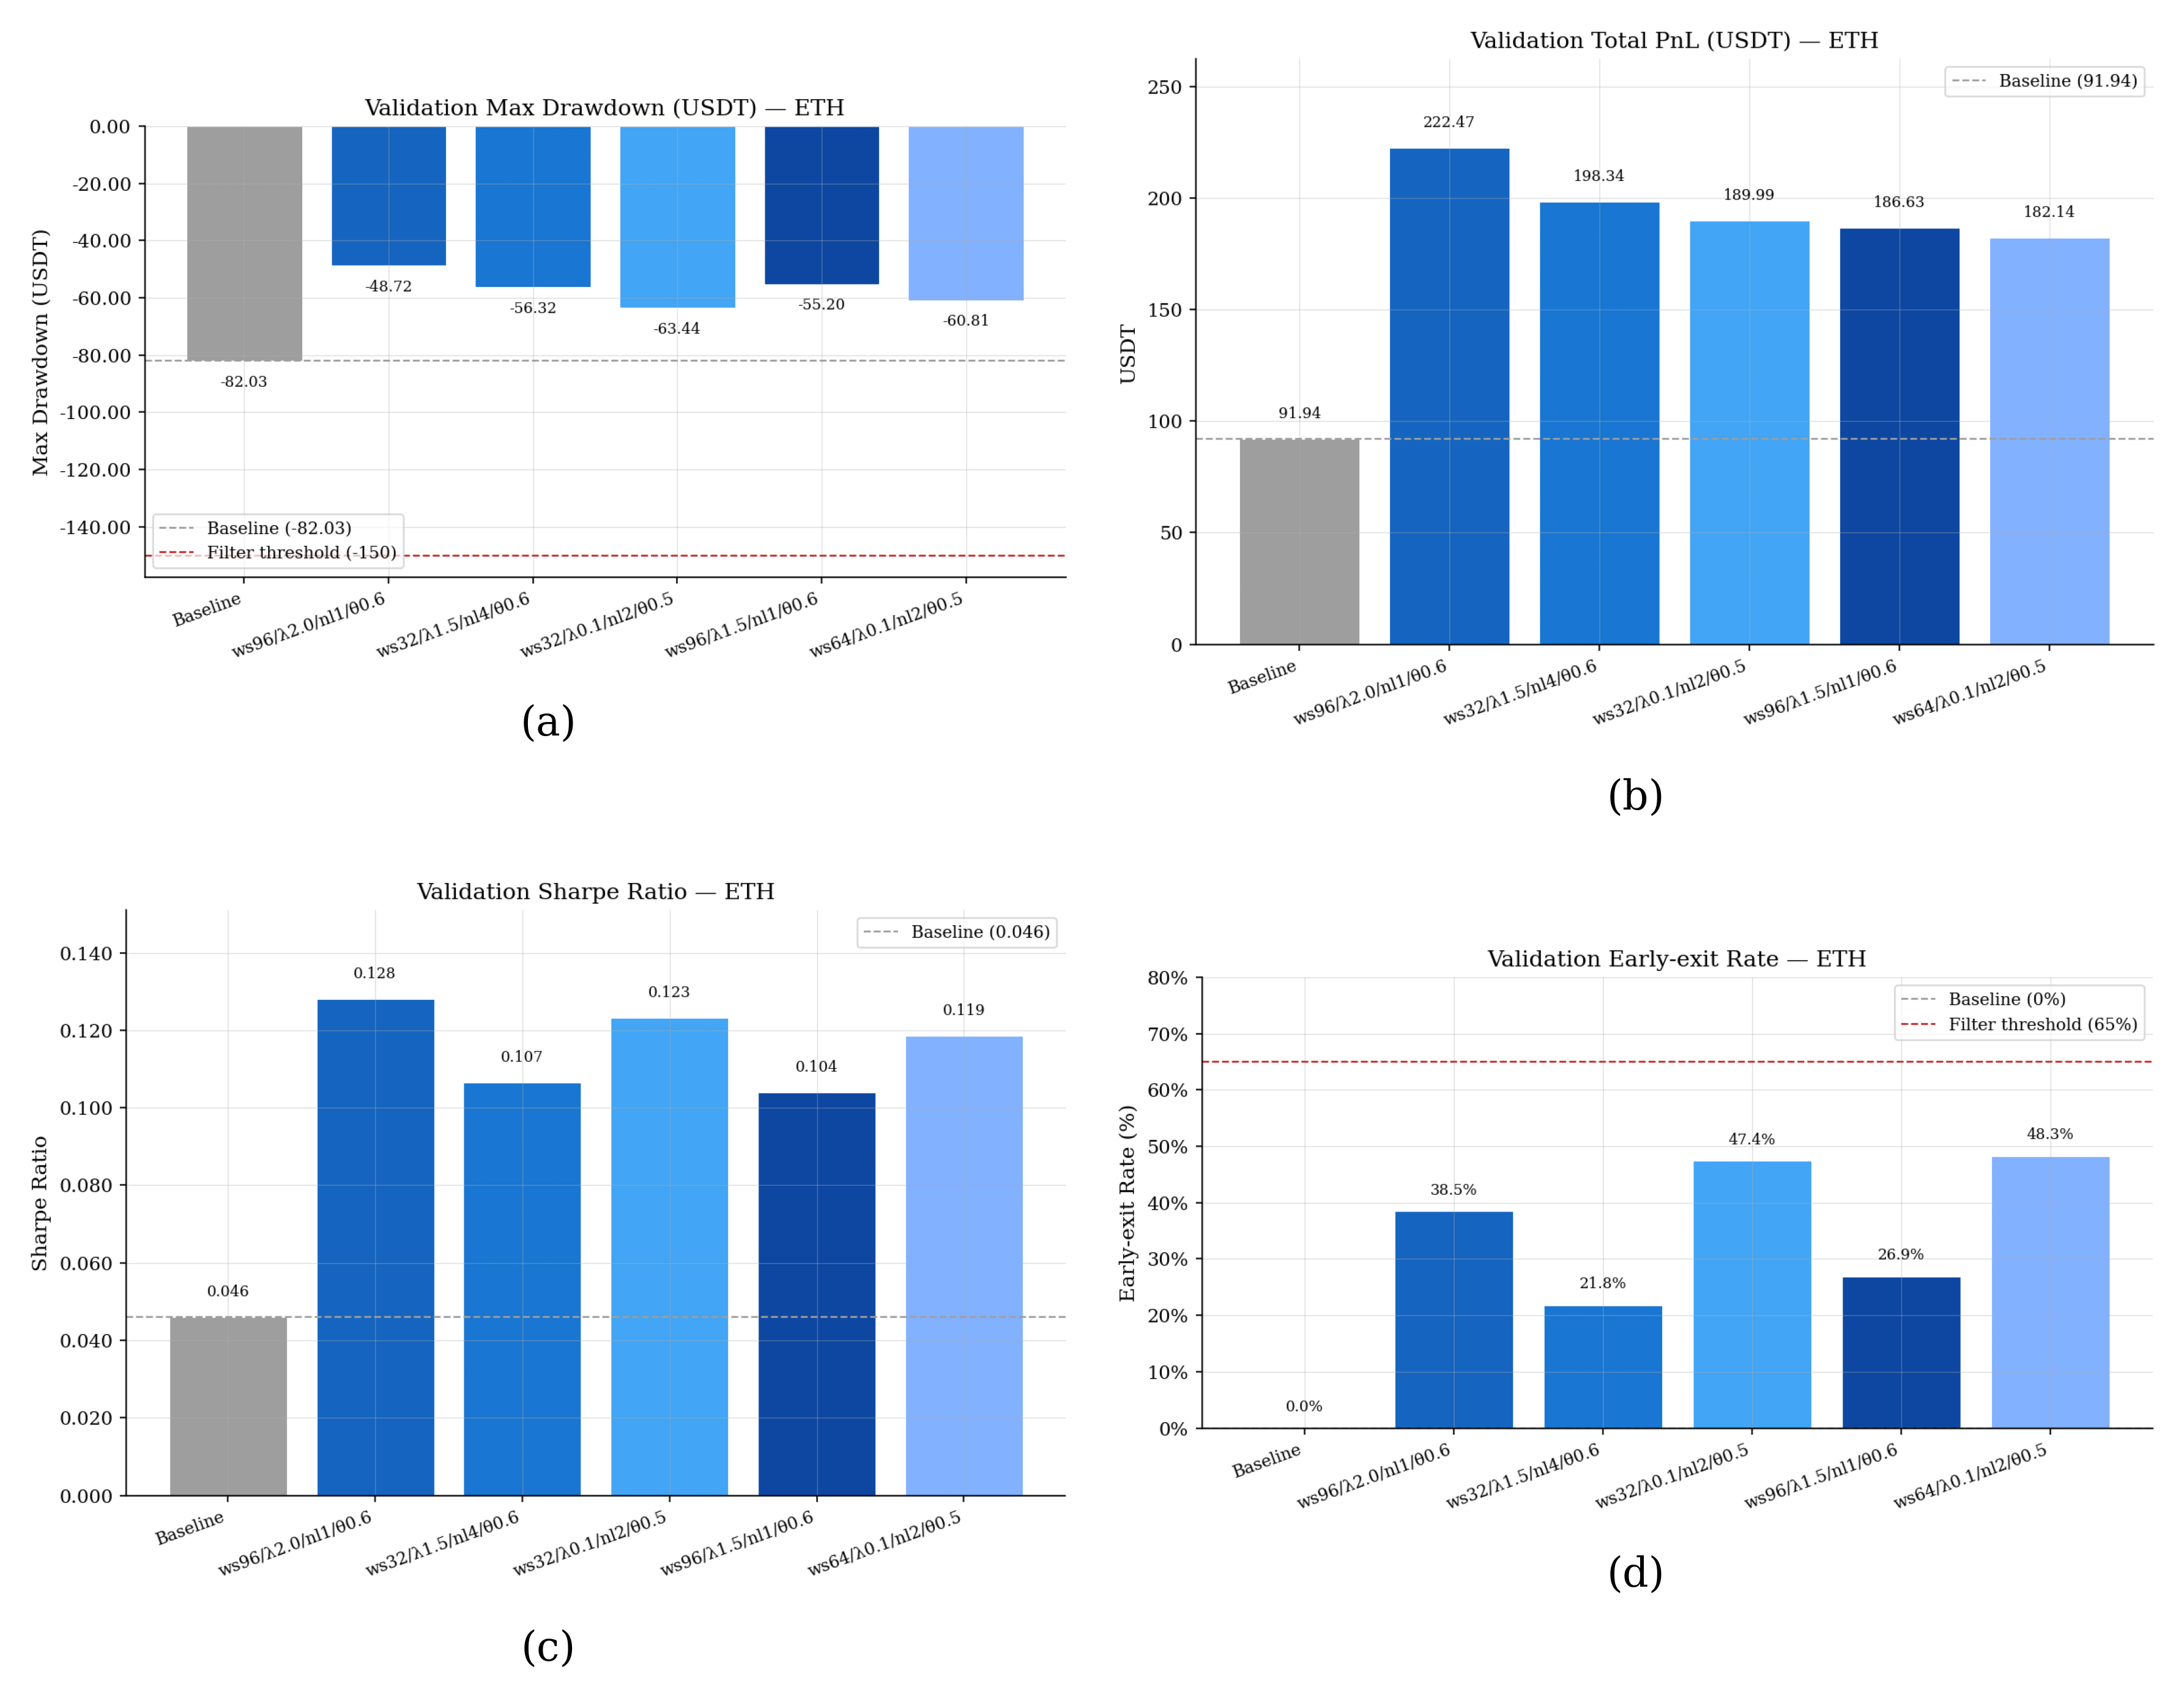
\includegraphics[width=0.85\textwidth]{figs/merged_val_eth.png}
    \caption{Validation Set Metrics of Top Five Models - ETH}  
    \label{fig:merged_val_eth}
    \vspace{6pt} 
    \parbox{0.85\textwidth}{\footnotesize \textit{Note:} This figure presents the validation set performance on ETH of the top five optimal parameter configurations for the LSTM early exit model. Specifically, Panel (a) depicts the maximum drawdown of the models, Panel (b) illustrates the average profitability, Panel (c) presents the Sharpe ratio, and Panel (d) shows the early exit trigger probability.}
\end{figure}

\begin{figure}[H]
    \centering
    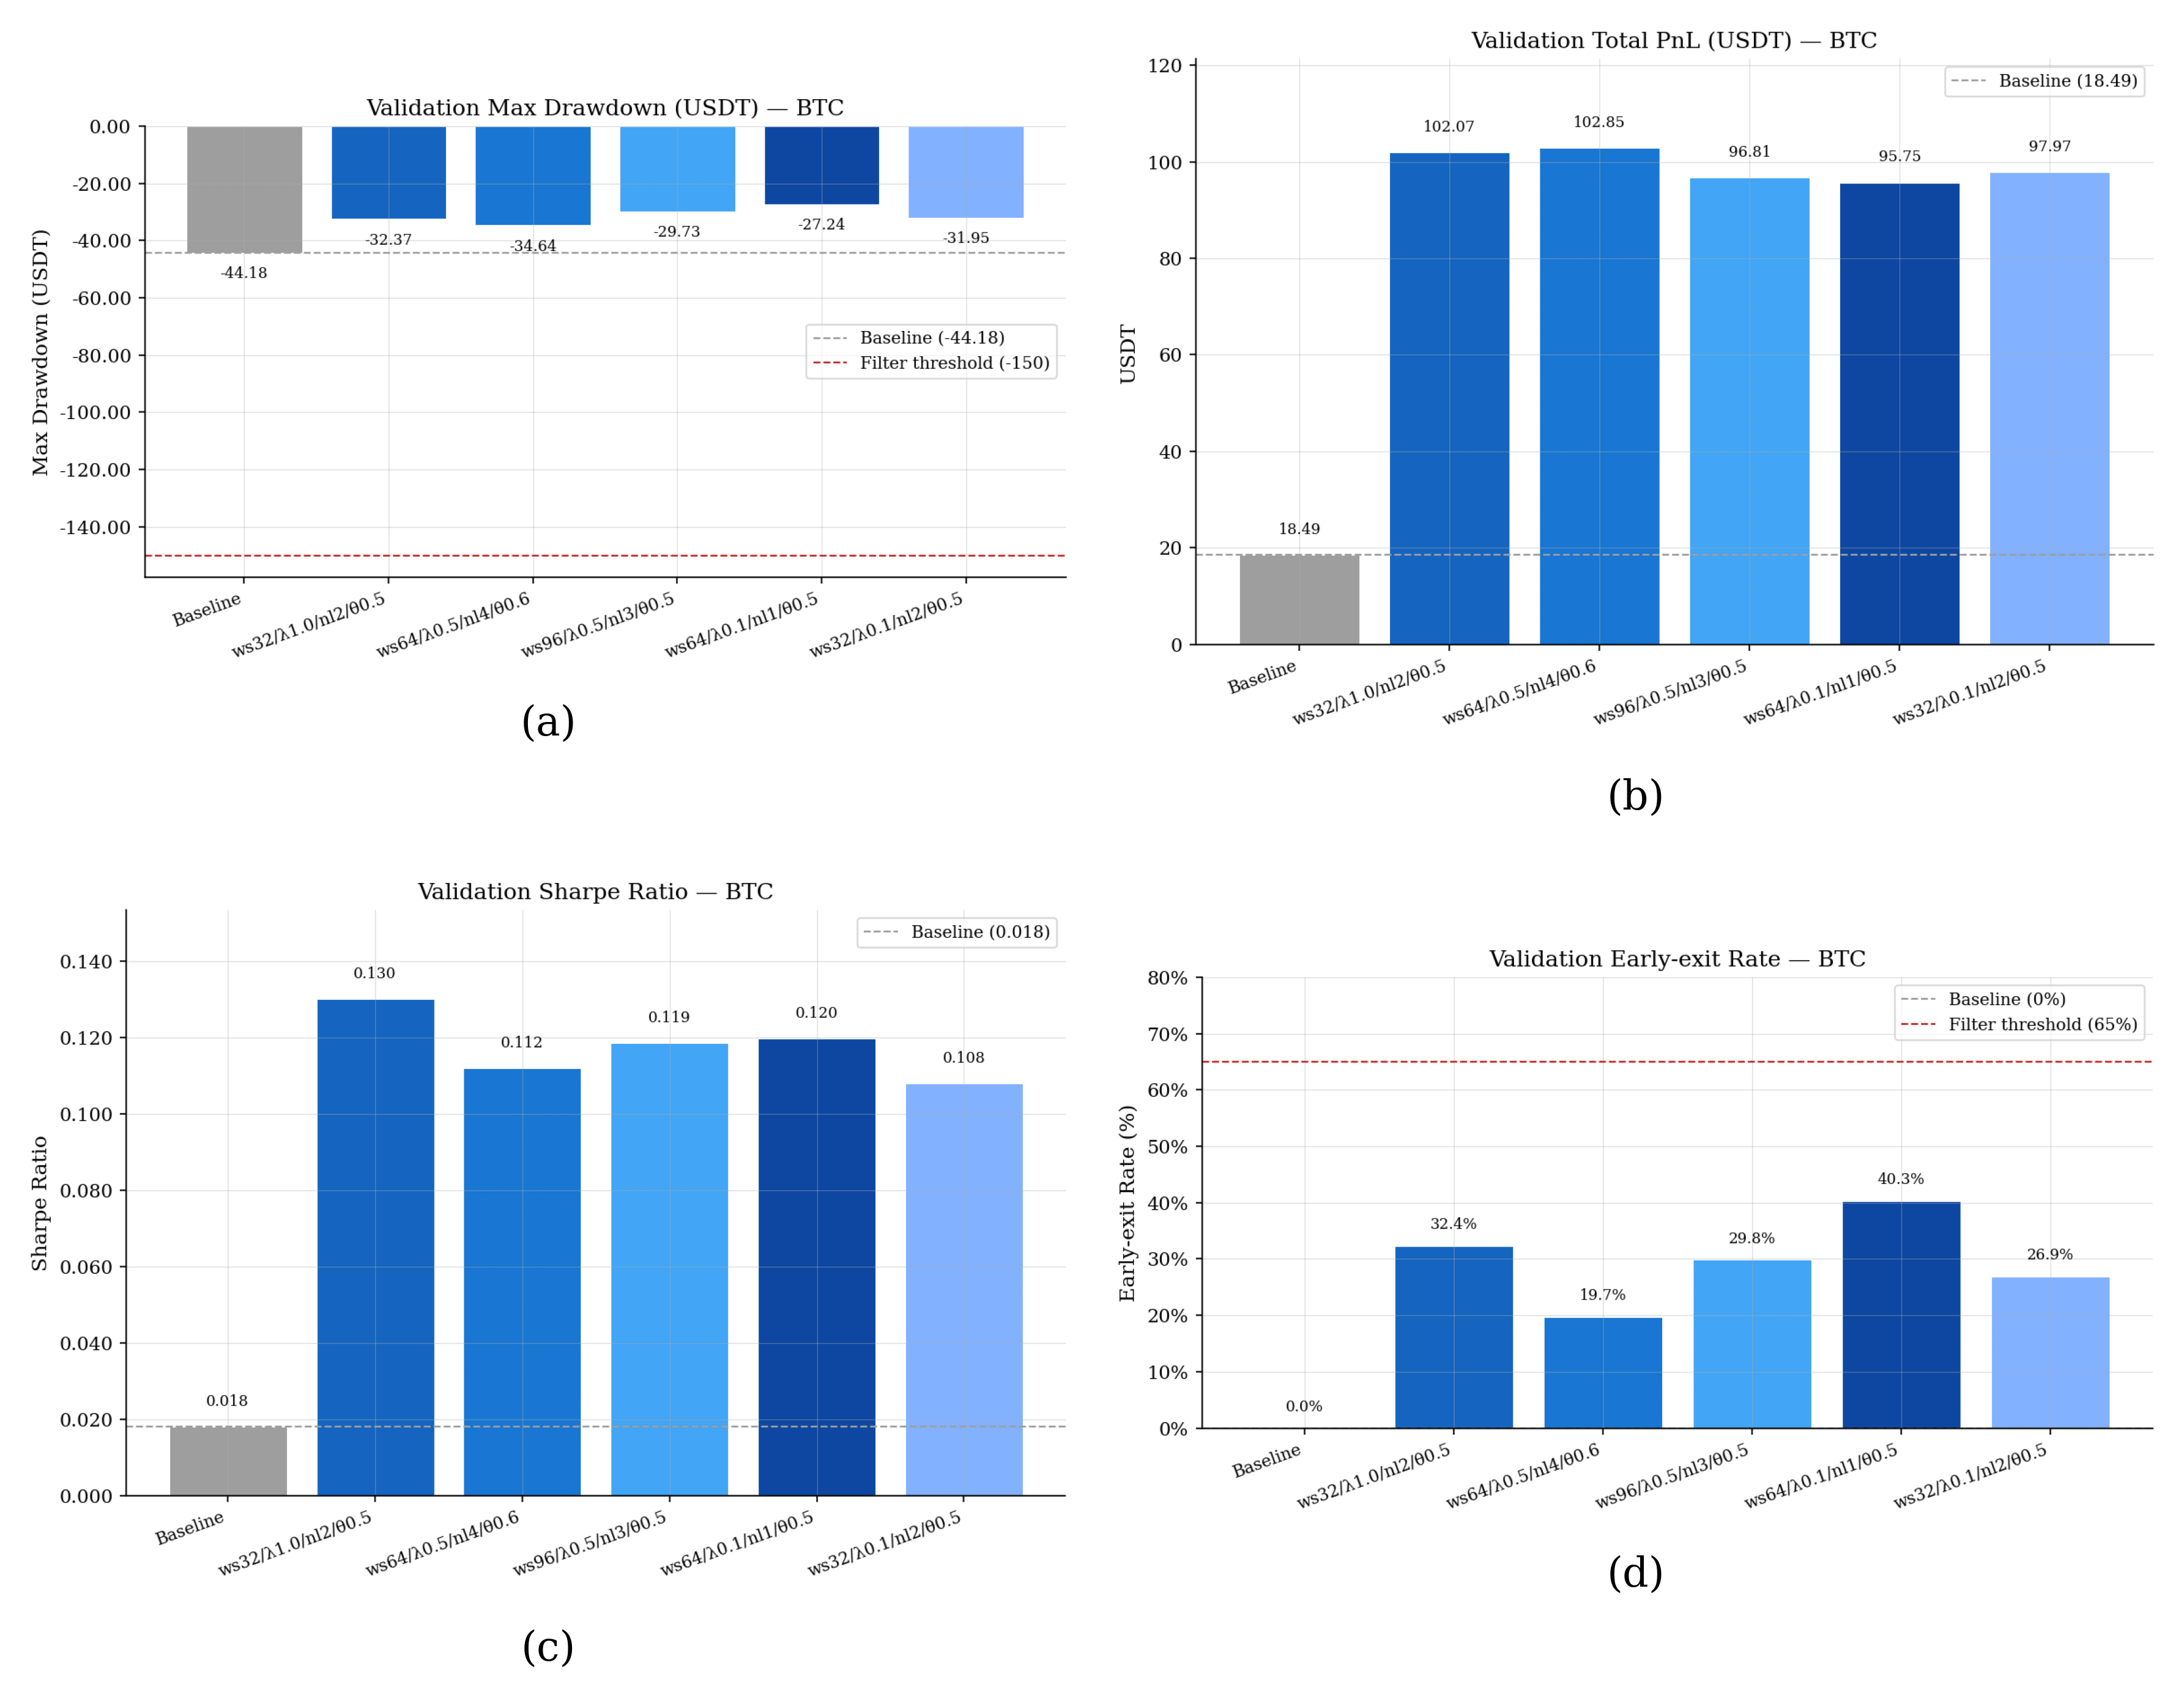
\includegraphics[width=0.85\textwidth]{figs/merged_val_btc.png}
    \caption{Validation Set Metrics of Top Five Models - BTC}  
    \label{fig:merged_val_btc}
    \vspace{6pt} 
    \parbox{0.85\textwidth}{\footnotesize \textit{Note:} This figure presents the validation set performance on BTC of the top five optimal parameter configurations for the LSTM early exit model. Specifically, Panel (a) depicts the maximum drawdown of the models, Panel (b) illustrates the average profitability, Panel (c) presents the Sharpe ratio, and Panel (d) shows the early exit trigger probability.}
\end{figure}

\begin{figure}[H]
    \centering
    \includegraphics[width=0.85\textwidth]{figs/merged_val_XRP.png}
    \caption{Validation Set Metrics of Top Five Models - XRP}  
    \label{fig:merged_val_XRP}
    \vspace{6pt} 
    \parbox{0.85\textwidth}{\footnotesize \textit{Note:} This figure presents the validation set performance on XRP of the top five optimal parameter configurations for the LSTM early exit model. Specifically, Panel (a) depicts the maximum drawdown of the models, Panel (b) illustrates the average profitability, Panel (c) presents the Sharpe ratio, and Panel (d) shows the early exit trigger probability.}
\end{figure}

\begin{figure}[H]
    \centering
    \includegraphics[width=0.85\textwidth]{figs/merged_val_SOL.png}
    \caption{Validation Set Metrics of Top Five Models - SOL}  
    \label{fig:merged_val_SOL}
    \vspace{6pt} 
    \parbox{0.85\textwidth}{\footnotesize \textit{Note:} This figure presents the validation set performance on SOL of the top five optimal parameter configurations for the LSTM early exit model. Specifically, Panel (a) depicts the maximum drawdown of the models, Panel (b) illustrates the average profitability, Panel (c) presents the Sharpe ratio, and Panel (d) shows the early exit trigger probability.}
\end{figure}

\subsection{Sensitivity Analysis}\label{subsec:sensitivityAnalysis}

\begin{figure}[H]
    \centering
    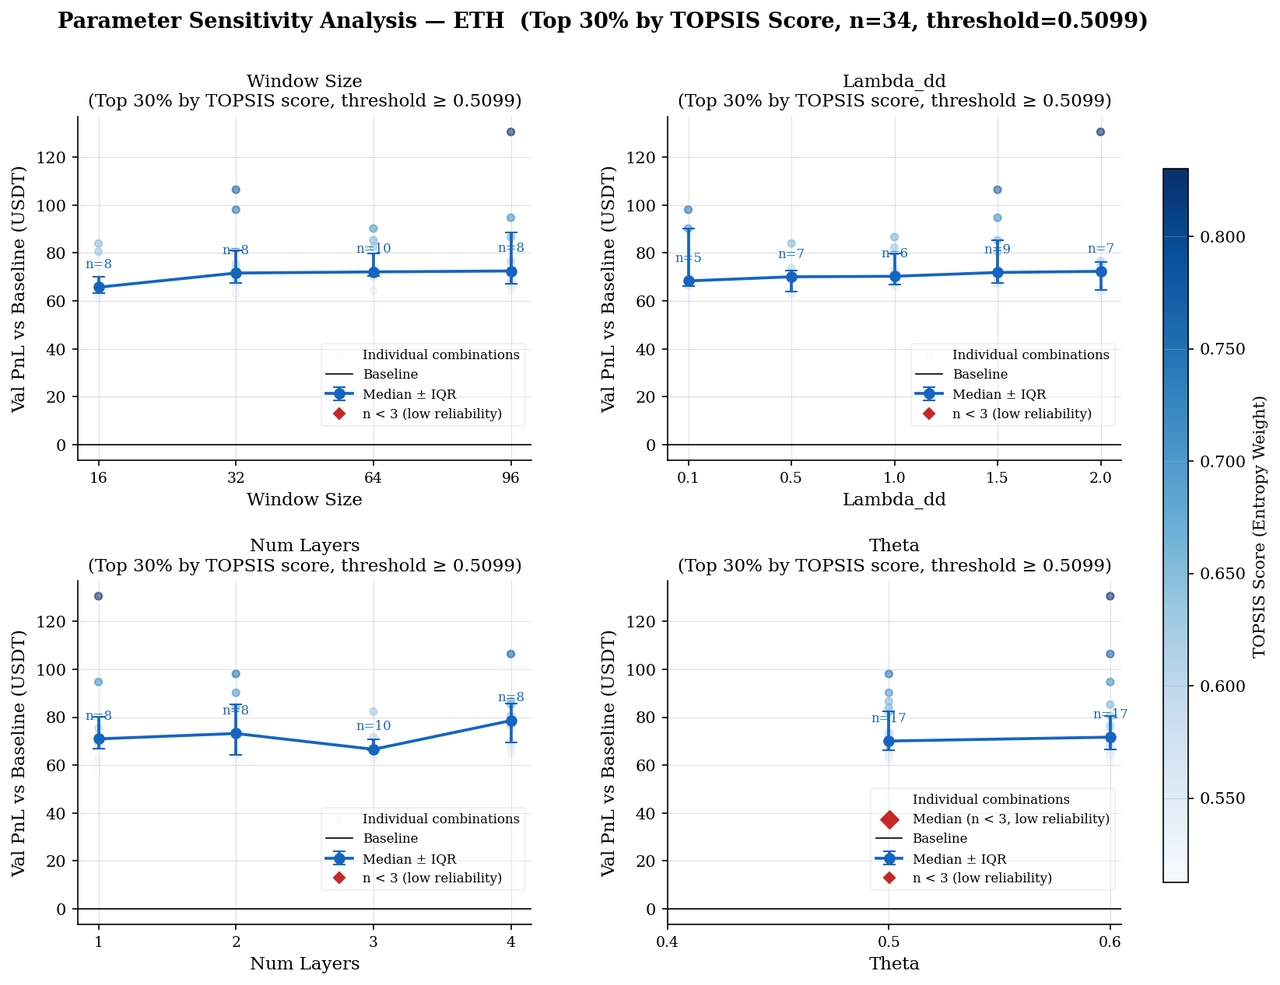
\includegraphics[width=0.85\textwidth]{figs/stest_eth.png}
    \caption{Sensitivity Analysis for Hyperparameters - ETH}  
    \label{fig:stest_eth}
    \vspace{6pt} 
    \parbox{0.85\textwidth}{\footnotesize \textit{Note:} This figure presents a sensitivity analysis of the hyperparameters in the LSTM early exit model for ETH, including the lookback window, the drawdown penalty coefficient, the number of neural network layers, and the early exit decision threshold $\theta$.}
\end{figure}

\begin{figure}[H]
    \centering
    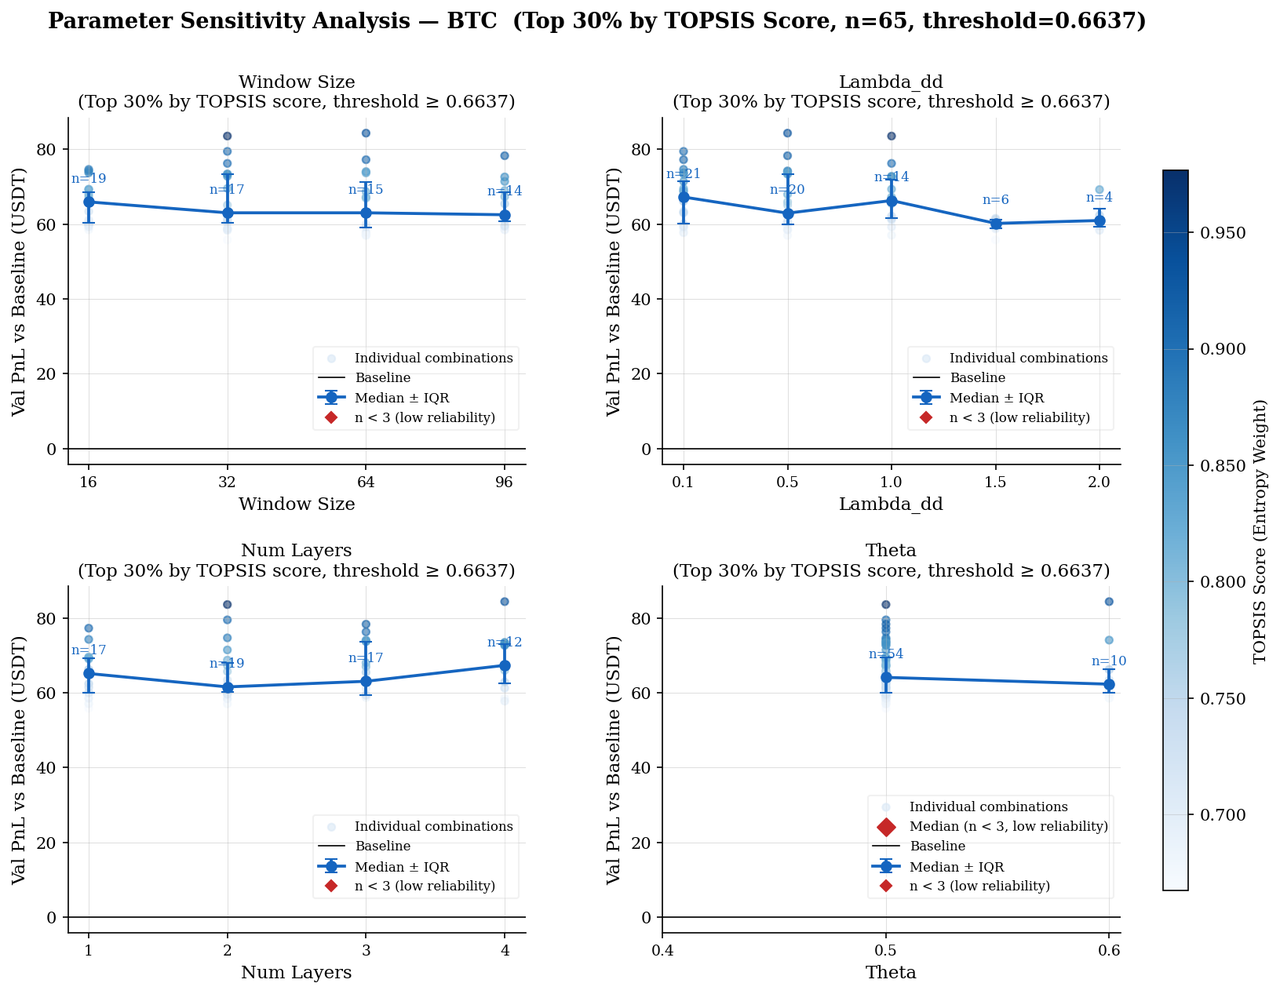
\includegraphics[width=0.85\textwidth]{figs/stest_btc.png}
    \caption{Sensitivity Analysis for Hyperparameters - BTC}  
    \label{fig:stest_btc}
    \vspace{6pt} 
    \parbox{0.85\textwidth}{\footnotesize \textit{Note:} This figure presents a sensitivity analysis of the hyperparameters in the LSTM early exit model for BTC, including the lookback window, the drawdown penalty coefficient, the number of neural network layers, and the early exit decision threshold $\theta$.}
\end{figure}

\begin{figure}[H]
    \centering
    \includegraphics[width=0.85\textwidth]{figs/stest_XRP.png}
    \caption{Sensitivity Analysis for Hyperparameters - XRP}  
    \label{fig:stest_XRP}
    \vspace{6pt} 
    \parbox{0.85\textwidth}{\footnotesize \textit{Note:} This figure presents a sensitivity analysis of the hyperparameters in the LSTM early exit model for XRP, including the lookback window, the drawdown penalty coefficient, the number of neural network layers, and the early exit decision threshold $\theta$.}
\end{figure}

\begin{figure}[H]
    \centering
    \includegraphics[width=0.85\textwidth]{figs/stest_SOL.png}
    \caption{Sensitivity Analysis for Hyperparameters - SOL}  
    \label{fig:stest_SOL}
    \vspace{6pt} 
    \parbox{0.85\textwidth}{\footnotesize \textit{Note:} This figure presents a sensitivity analysis of the hyperparameters in the LSTM early exit model for SOL, including the lookback window, the drawdown penalty coefficient, the number of neural network layers, and the early exit decision threshold $\theta$.}
\end{figure}





% \setcounter{figure}{0}
% \renewcommand{\thefigure}{\Alph{section}.\arabic{figure}}
% \begin{figure}[H]
%     \centering
%     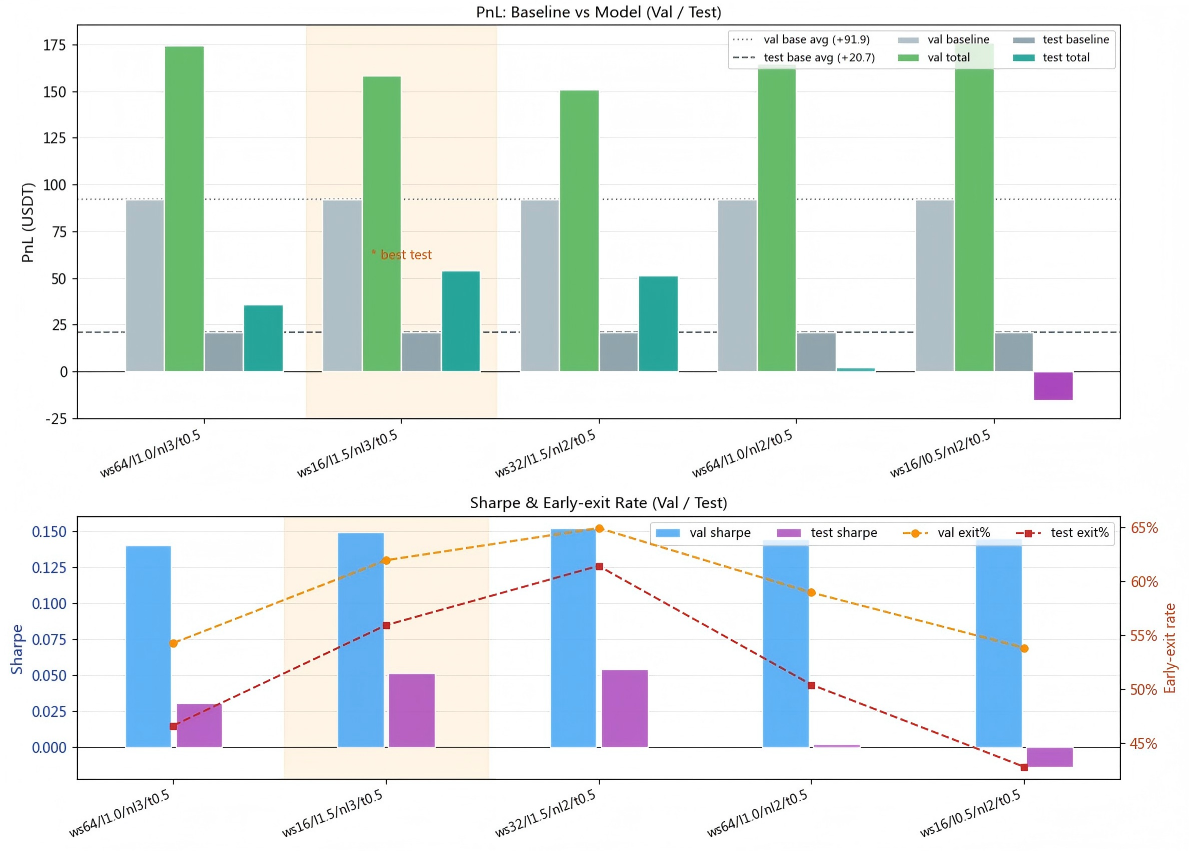
\includegraphics[width=0.85\textwidth]{figs/gridsearch_eth.png}
%     \caption{Grid Search:Val vs Test Metrics - ETH}
%     \label{fig:gridsearch_val_eth}
%     \vspace{6pt} 
%     \parbox{\textwidth}{\footnotesize \textit{Note:} 上方的图展示的是基准策略与模型在}
% \end{figure}

% \subsection{Ablation Analysis for Label Margin}\label{subsec:ablationAnalysis}

% \begin{figure}[H]
%     \centering
%     
\includegraphics[width=0.85\textwidth]{figs/labelmargin_eth.png}
%     \caption{Label Margin Effect - ETH}
%     \label{fig:labelmargin_eth}
%     \vspace{6pt} 
%     \parbox{\textwidth}{\footnotesize \textit{Note:} The different colored lines represent the variation of the model's performance metrics across varying $\Delta_{\text{margin}}$ under distinct parameter combinations, while the gray vertical dashed line indicates the initial label margin value. The upper panel displays the profitability level, and the lower panel presents the positive sample ratio.}
% \end{figure}

% \begin{figure}[H]
%     \centering
%     
\includegraphics[width=0.85\textwidth]{figs/labelmargin_btc.png}
%     \caption{Label Margin Effect - BTC}
%     \label{fig:labelmargin_btc}
%     \vspace{6pt} 
%     \parbox{\textwidth}{\footnotesize \textit{Note:} The different colored lines represent the variation of the model's performance metrics across varying $\Delta_{\text{margin}}$ under distinct parameter combinations, while the gray vertical dashed line indicates the initial label margin value. The upper panel displays the profitability level, and the lower panel presents the positive sample ratio.}
% \end{figure}

% \begin{figure}[H]
%     \centering
%     
\includegraphics[width=0.85\textwidth]{figs/labelmargin_xrp.png}
%     \caption{Label Margin Effect - XRP}
%     \label{fig:labelmargin_xrp}
%     \vspace{6pt} 
%     \parbox{\textwidth}{\footnotesize \textit{Note:} The different colored lines represent the variation of the model's performance metrics across varying $\Delta_{\text{margin}}$ under distinct parameter combinations, while the gray vertical dashed line indicates the initial label margin value. The upper panel displays the profitability level, and the lower panel presents the positive sample ratio.}
% \end{figure}

% \begin{figure}[H]
%     \centering
%     
\includegraphics[width=0.85\textwidth]{figs/labelmargin_sol.png}
%     \caption{Label Margin Effect - SOL}
%     \label{fig:labelmargin_sol}
%     \vspace{6pt} 
%     \parbox{\textwidth}{\footnotesize \textit{Note:} The different colored lines represent the variation of the model's performance metrics across varying $\Delta_{\text{margin}}$ under distinct parameter combinations, while the gray vertical dashed line indicates the initial label margin value. The upper panel displays the profitability level, and the lower panel presents the positive sample ratio.}
% \end{figure}

% \subsection{LSTM Early Stopping Details}\label{subsec:LSTM_Early_Stopping_Details}

% \begin{figure}[H]
%     \centering
%     
\includegraphics[width=0.85\textwidth]{figs/eth_cummupnl_each.png}
%     \caption{Cumulative Returns of Different Strategies and early exit Models for ETH}
%     \label{fig:eth_each_pnl}
%     \vspace{6pt} 
%     \parbox{0.85\textwidth}{\footnotesize \textit{Note:} This figure illustrates the cumulative returns for the ETH asset under the three different LSTM early exit models, the baseline WMA strategy, and the buy-and-hold strategy. The solid blue lines represent the LSTM early exit models under distinct parameter configurations, the dashed line represents the baseline WMA strategy, and the solid orange line represents the buy-and-hold strategy.}
% \end{figure}

% \begin{figure}[H]
%     \centering
%     
\includegraphics[width=0.85\textwidth]{figs/btc_cummupnl_each.png}
%     \caption{Cumulative Returns of Different Strategies and early exit Models for BTC}
%     \label{fig:btc_each_pnl}
%     \vspace{6pt} 
%     \parbox{0.85\textwidth}{\footnotesize \textit{Note:} This figure illustrates the cumulative returns for the BTC asset under the three different LSTM early exit models, the baseline WMA strategy, and the buy-and-hold strategy. The solid blue lines represent the LSTM early exit models under distinct parameter configurations, the dashed line represents the baseline WMA strategy, and the solid orange line represents the buy-and-hold strategy.}
% \end{figure}

% \begin{figure}[H]
%     \centering
%     
\includegraphics[width=0.85\textwidth]{figs/xrp_cummupnl_each.png}
%     \caption{Cumulative Returns of Different Strategies and early exit Models for XRP}
%     \label{fig:xrp_each_pnl}
%     \vspace{6pt} 
%     \parbox{0.85\textwidth}{\footnotesize \textit{Note:} This figure illustrates the cumulative returns for the XRP asset under the three different LSTM early exit models, the baseline WMA strategy, and the buy-and-hold strategy. The solid blue lines represent the LSTM early exit models under distinct parameter configurations, the dashed line represents the baseline WMA strategy, and the solid orange line represents the buy-and-hold strategy.}
% \end{figure}

% \begin{figure}[H]
%     \centering
%     
\includegraphics[width=0.85\textwidth]{figs/sol_cummupnl_each.png}
%     \caption{Cumulative Returns of Different Strategies and early exit Models for SOL}
%     \label{fig:sol_each_pnl}
%     \vspace{6pt} 
%     \parbox{0.85\textwidth}{\footnotesize \textit{Note:} This figure illustrates the cumulative returns for the SOL asset under the three different LSTM early exit models, the baseline WMA strategy, and the buy-and-hold strategy. The solid blue lines represent the LSTM early exit models under distinct parameter configurations, the dashed line represents the baseline WMA strategy, and the solid orange line represents the buy-and-hold strategy.}
% \end{figure}

% \subsection{Test Set Metrics}\label{subsec:Test_Set_Metrics}

% \begin{figure}[H]
%     \centering
%     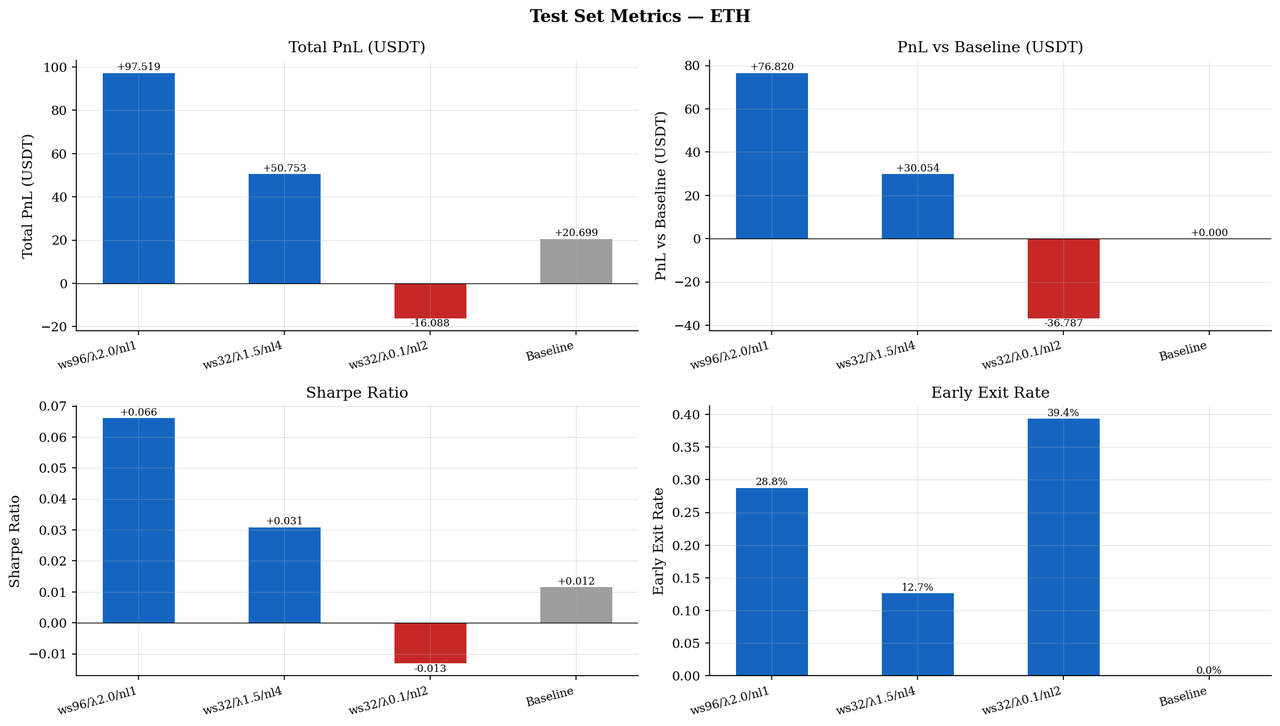
\includegraphics[width=0.85\textwidth]{figs/eth_test_metrics.png}
%     \caption{Test Set Metrics for ETH}
%     \label{fig:eth_test_metrics}
%     \vspace{6pt} 
%     \parbox{0.85\textwidth}{\footnotesize \textit{Note:} This figure presents the performance evaluation metrics on the test set for the top three optimal LSTM early exit strategies and the baseline WMA strategy applied to ETH. The four panels illustrate, respectively, the cumulative returns, the relative cumulative returns against the baseline strategy, the Sharpe ratio, and the early exit probability across the different strategies.}
% \end{figure}

% \begin{figure}[H]
%     \centering
%     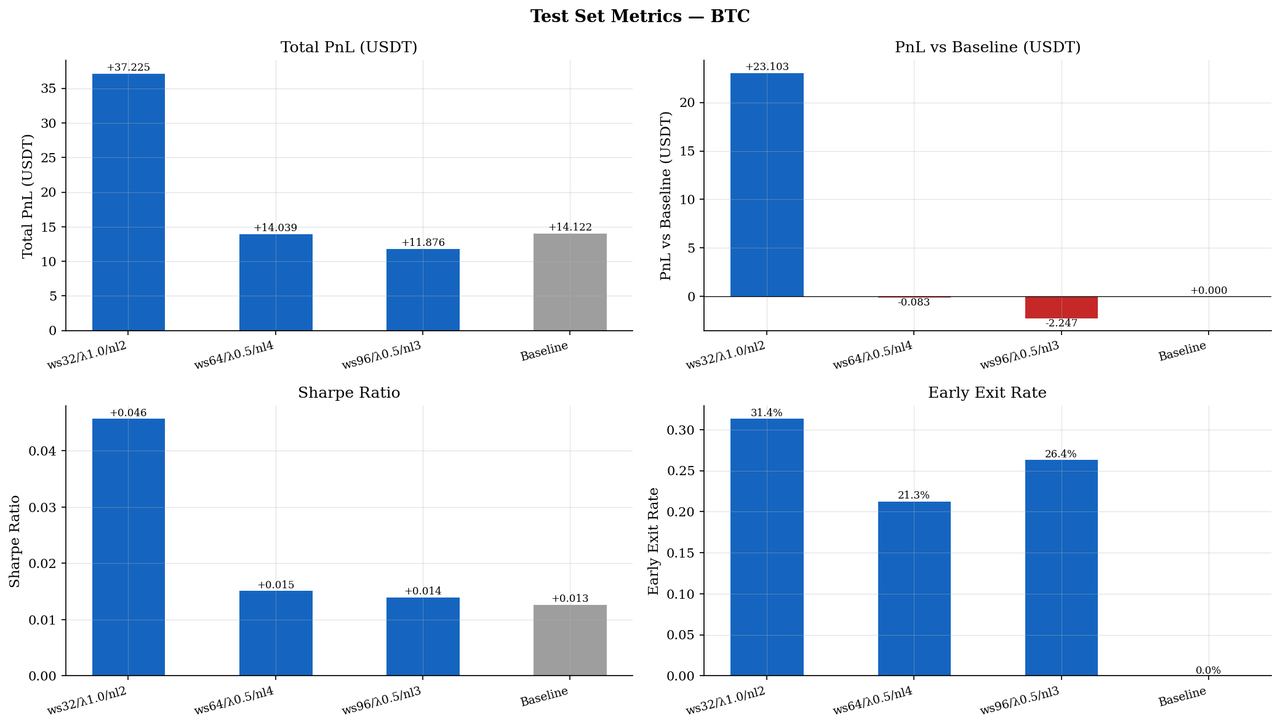
\includegraphics[width=0.85\textwidth]{figs/btc_test_metrics.png}
%     \caption{Test Set Metrics for BTC}
%     \label{fig:btc_test_metrics}
%     \vspace{6pt} 
%     \parbox{0.85\textwidth}{\footnotesize \textit{Note:} This figure presents the performance evaluation metrics on the test set for the top three optimal LSTM early exit strategies and the baseline WMA strategy applied to BTC. The four panels illustrate, respectively, the cumulative returns, the relative cumulative returns against the baseline strategy, the Sharpe ratio, and the early exit probability across the different strategies.}
% \end{figure}

% \begin{figure}[H]
%     \centering
%     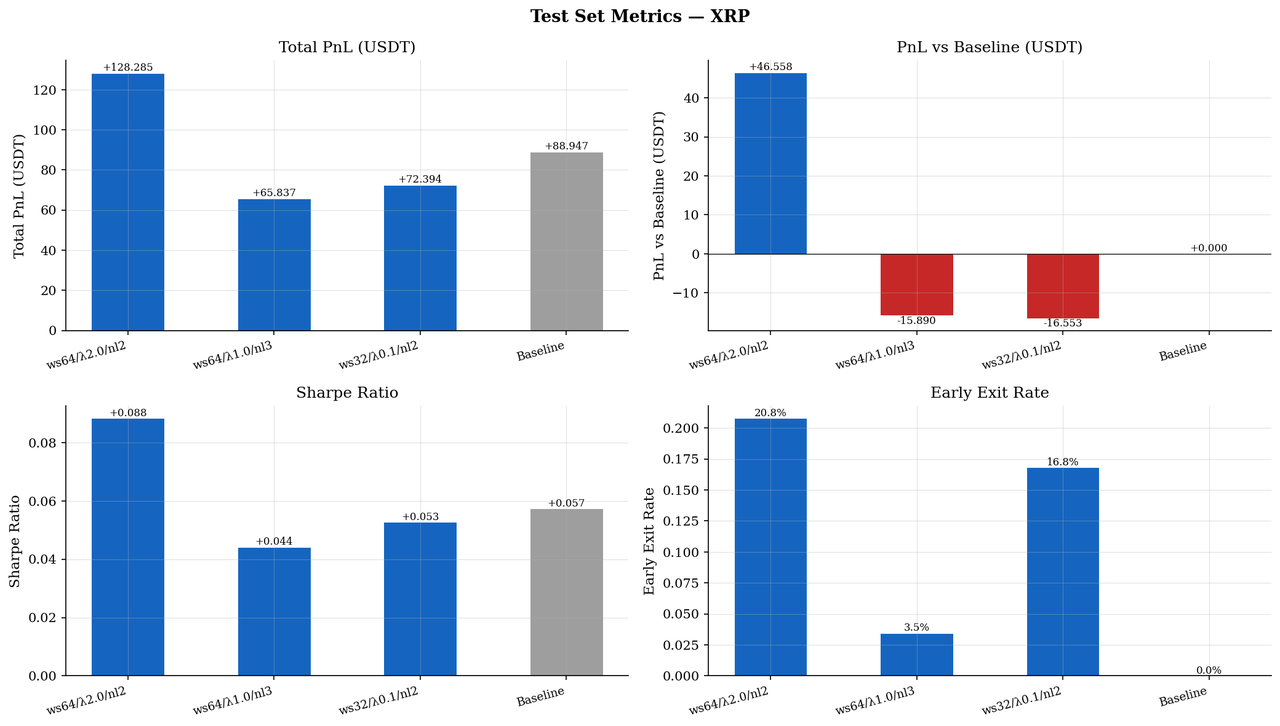
\includegraphics[width=0.85\textwidth]{figs/xrp_test_metrics.png}
%     \caption{Test Set Metrics for XRP}
%     \label{fig:xrp_test_metrics}
%     \vspace{6pt} 
%     \parbox{0.85\textwidth}{\footnotesize \textit{Note:} This figure presents the performance evaluation metrics on the test set for the top three optimal LSTM early exit strategies and the baseline WMA strategy applied to XRP. The four panels illustrate, respectively, the cumulative returns, the relative cumulative returns against the baseline strategy, the Sharpe ratio, and the early exit probability across the different strategies.}
% \end{figure}

% \begin{figure}[H]
%     \centering
%     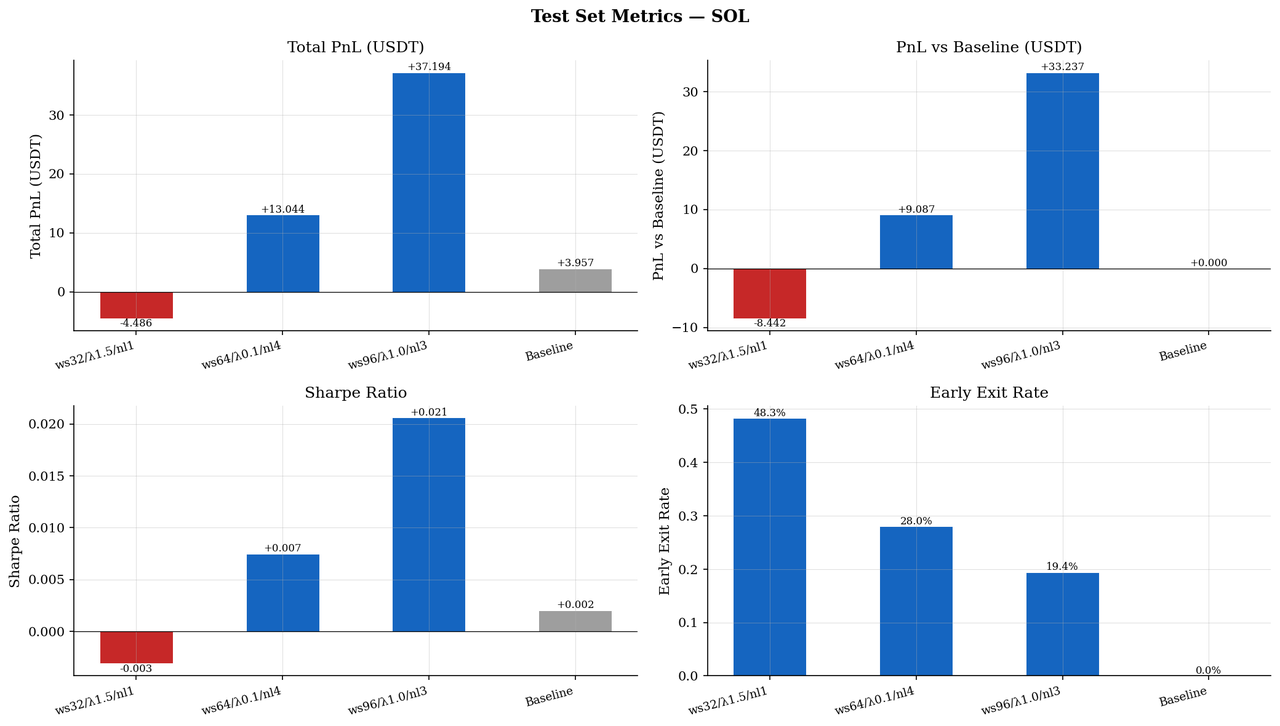
\includegraphics[width=0.85\textwidth]{figs/sol_test_metrics.png}
%     \caption{Test Set Metrics for SOL}
%     \label{fig:sol_test_metrics}
%     \vspace{6pt} 
%     \parbox{0.85\textwidth}{\footnotesize \textit{Note:} This figure presents the performance evaluation metrics on the test set for the top three optimal LSTM early exit strategies and the baseline WMA strategy applied to SOL. The four panels illustrate, respectively, the cumulative returns, the relative cumulative returns against the baseline strategy, the Sharpe ratio, and the early exit probability across the different strategies.}
% \end{figure}

% Additional figures can be placed here.

\end{document}